\documentclass[a4paper,twoside,12pt]{book}
\usepackage[T1]{fontenc} 
\usepackage[utf8]{inputenc}   
\usepackage[czech]{babel} 
%\usepackage[a4paper, hmarginratio=3:2]{geometry} 
\usepackage[a4paper, inner=3.5cm, textwidth=15cm, top=2.5cm, textheight=24cm]{geometry} 
\usepackage{pdfpages} % pokud nemáte formulář "Zadání bak./dipl. práce" naskenovaný jako PDF, tak ZAKOMENTUJTE
\usepackage[hidelinks]{hyperref} % v PDF budou klikací odkazy ("hidelinks" je nebude rámovat)

\usepackage{graphicx} 
\usepackage{epsfig} 
\usepackage{float} 
\usepackage{caption} 
\usepackage{tabularx} 
\usepackage{listings}  
\usepackage{amsmath} 
\usepackage{cite}

\frenchspacing % za~větou bude mezislovní mezera (v anglických textech je mezera za~větou delší)
\widowpenalty=1000 % "síla" zákazu vdov (= jeden řádek ze~začátku odstavce na~konci stránky)
\clubpenalty=1000 % "síla" zákazu sirotků (= jeden řádek/slovo z konce odstavce samostatně na~začátku stránky)
\brokenpenalty=1000 % "síla" zákazu zlomu stránky za~řádkem, který má na~konci rozdělené slovo


\usepackage{parskip}
%\usepackage{indentfirst}
\pagenumbering{arabic} % číslování stránek arabskými číslicemi
\pagestyle{plain}      % stránky číslované do~le uprostřed

%----------------------------------------------------------------------------------------
%	TITLE SECTION
%----------------------------------------------------------------------------------------

\newcommand{\horrule}[1]{\rule{\linewidth}{#1}} % Create horizontal rule command with 1 argument of height

\newcommand{\cvut}{ČESKÉ VYSOKÉ UČENÍ TECHNICKÉ
V~PRAZE}
\newcommand{\nazevcz}{Elektronové dělo a detekce elektronového svazku}
\newcommand{\fjfi}{Fakulta jaderná a fyzikálně inženýrská}
\newcommand{\kf}{Katedra Fyziky} 
\newcommand{\logoCVUT}{
\includegraphics{symbol_cvut_konturova_verze_cb.pdf}}



\begin{document}
%\nocite{*}

\newpage 
\thispagestyle{empty}

\begin{center}
	{\LARGE
		\cvut\par
		\fjfi
	}
    \vspace{10mm}

   \vspace{10mm} \logoCVUT \vspace{15mm} 

   {\huge \textbf{\nazevcz}\par}
   
   \vspace{15mm}
   
   Ekaterina Eremenko, Anežka Kabátová, Jakub Kubát, \\
Tomáš Novák, Monika Robotková, Jaroslav Štorek, \\
Tomáš Truhlář, Matěj Vaculčiak

\vspace{15mm}

\normalsize\today

\end{center}


\newpage 
\thispagestyle{empty}

{\Large
	\textbf{Členové kolaborace}
}

\vspace{5mm}

\begin{center}
\textbf{Koordinátor projektu} \\
Tomáš Truhlář 

    \vspace{5mm}
    
\textbf{Mluvčí projektu} \\
Anežka Kabátová \\

\vspace{3mm}

***

\vspace{3mm}

\textbf{Konstrukce elektronového děl}a \\
Monika Robotková\\
Jaroslav Štorek\\
Tomáš Novák\\
Tomáš Truhlář

   \vspace{5mm}
   
\textbf{Fokusace elektronového svazk}u \\
Ekaterina Eremenko\\
Jakub Kubát


\vspace{5mm}

\textbf{Měření elektronového svazku} \\
Anežka Kabátová \\
Matěj Vaculčiak


\end{center}

\newpage  
\parskip=0pt
\tableofcontents 
\parskip=7pt
\newpage 
\listoffigures
\newpage
\listoftables
\newpage

\newpage
\newpage
\chapter*{Úvod} % normalni kapitola \chapter{kapitola}
\addcontentsline{toc}{chapter}{Úvod}

Za úkol na předmětu Projektové Praktikum bylo zadáno navrhnout a následně sestrojit aparaturu pro urychlování svazku elektronů a zařízení pro jejich detekci, což zahrnuje návrh a realizaci zapojení elektronového děla, zdroje vysokého napětí, doplňující soustavu fokusující svazek a v neposlední řadě samotný detektor intenzity elektronového svazku. 

Hned v úvodu jsme se tedy rozdělili na tři podskupiny, z nichž jedna se zabývala samotnou konstrukcí děla, jeho instalací do vakuové komory a zprovozněním urychlovací soustavy. Druhá skupina se zaměřila na fokusaci svazku elektronů, která spočívala v nalezení ideální konfigurace fokusovacích diod na základě simulací v programu SIMION. Třetí skupina se zabývala výrobou detektoru pro měření intenzity elektronového svazku, připojení vyčítacího zařízení a následné zpracování a analýza naměřených dat.

Na začátku projektu jsme se rozhodli, že se pokusíme vytvořit elektronový svazek o energii zhruba 80 keV, aby bylo možné použít monolitický pixelový detektor, který jsme si byli schopni sami sestrojit. První pokusy vytvořit elektronový svazek se žhaveným wolframovým vláknem jako zdrojem elektronů však nebyly úspěšné a později jsme přešli k průmyslovému elektronovému dělu. Svazek jsme urychlovali měděnými elektrodami. Z důvodu pozorovaných elektrických výbojů jsme nebyli na elektrodách schopni dosáhnout zamýšleného potenciálového rozdílu 80 kV, nýbrž jen 18 kV. K detekci signálu jsme proto použili destičku ze slitiny mědi a zlata, která konvertovala elektrony na námi detekovatelné fotony, a analyzovali výsledek měření.

První kapitola poskytuje teoretický úvod o elektronech a jejich chování v prostředí se sníženým tlakem. Je zde také popsán princip katodového záření a možnosti vedení elektrického proudu ve vakuu. 

Druhá kapitola pojednává o základních principech vzniku elektrických výbojů a jejich dělením. Druhá část této kapitoly se věnuje problematice vzniku elektrických výbojů v našem experimentu a popisuje způsoby, kterými jsme se snažili výbojům zamezit a předejít.

Třetí kapitola se zabývá principem fungování elektronového děla a emisí elektronů. Dále je zde popsáno sestavení vlastního elektronového děla a jeho technické parametry.

Ve čtvrté kapitole je představen zdroj elektronů ES40-PS, kterým bylo v pozdější fázi projektu nahrazeno naše původní elektronové dělo. V kapitole jsou rozepsány především technické detaily tohoto zdroje a jeho správné ovládání.

Pátá a šestá kapitola jsou věnovány fokusaci elektronového svazku. První ze zmiňovaných kapitol se zabývá především teorií samotné fokusace. Druhá zmíněná kapitola pak představuje simulační program SIMION a jeho konkrétní využití v našem experimentu.

Předposlední kapitola popisuje principy detekce elektronů a představuje detektor použitý v našem experimentu, jeho výrobu a technické parametry.

V poslední kapitole je uvedena metodika měřením, naměřená data a výsledky analýzy dat.


\newpage
\chapter{Elektrony a vakuum}
Před samotným započetím sestavování experimentu bylo nejdříve nutné pochopit podstatu chování elektronů při sníženém tlaku. Teprve pak bylo možné fokusovací a urychlovací aparaturu sestrojit. Tato kapitola se tedy věnuje základní charakteristice elektronů a jejich pohybu v prostředí se sníženým tlakem.

\section{Elektron}
Elektron je elementární částice se záporným elektrickým nábojem, která tvoří obal atomového jádra. V rámci Standardního modelu řadíme elektron do první generace skupiny leptonů. Jeho klidová hmotnost je $m_{0}=0,510~\mathrm{MeV}/c$ \cite{01Elektron} a spin 1/2. Poloviční spin jej řadí mezi fermiony, takže podléhá Pauliho vylučovacímu principu.

Elektrony jsou nositeli náboje při vedení elektrického proudu a také tvoří $\beta^{-}$ záření.

Elektron byl poprvé popsán v roce 1897 britským fyzikem J. J. Thomsonem, který takto vysvětlil podstatu katodového záření. Toto záření ale bylo pozorováno už v polovině 19. století W. Crooksem a několika dalšími fyziky. Experiment byl tvořen skleněnou (katodovou) trubicí s elektrodami naplněnou vzduchem nebo jiným plynem. Pokud byl v trubici dostatečně nízký tlak (asi tisícina atmosférického tlaku) a na elektrody bylo přivedeno vysoké napětí (více než 1000 V), objevilo se v trubici záření. Při dalším snižování tlaku bylo možné záření pozorovat i na stěně trubice, která se nacházela naproti katodě. Toto záření bylo označeno jako katodové záření a později Thomsonem popsáno jako proud elektronů.

\section{Katodové záření}
Katodové záření vzniká ve skleněné trubici se dvěma elektrodami. V této katodové trubici, ve které se nachází zředěný plyn, dochází při přivedení napětí na elektrody a postupném snižování tlaku k různým efektům spojeným s pohybem částic. Při tlaku zhruba 5 300 Pa se v trubici objevuje úzký sloupec vlnící se červený sloupec, který vychází z anody a končí těsně před katodou. Při dalším ředění plynu se sloupec rozšiřuje a zkracuje a vzniká tzv. anodový sloupec, který je od katody oddělen tmavým tzv. Faradayovým prostorem. Na katodě přitom vzniká doutnavé katodové světlo. Budeme-li se zřeďováním pokračovat, bude anodový sloupec v trubici blednout a stávat se vrstevnatým. Katodové světlo pak pokrývá celou katodu. Pokud dosáhneme hranici tlaku zhruba 2,67 Pa, molekuly plynu již v trubici nepřekážejí pohybu elektronů a iontů, které se pak šíří prostorem přímočaře a s velkou rychlostí. Veškeré světelné úkazy pak v trubici mizí a dochází pouze k fluorescenci stěn trubice. Fluorescence je vyvolána proudem elektronů letících z katody, jinak nazývaných katodové záření. Jednotlivé fáze zřeďování plynu jsou na Obr. \ref{01katody}

\begin{figure}[htbp!]
\centering
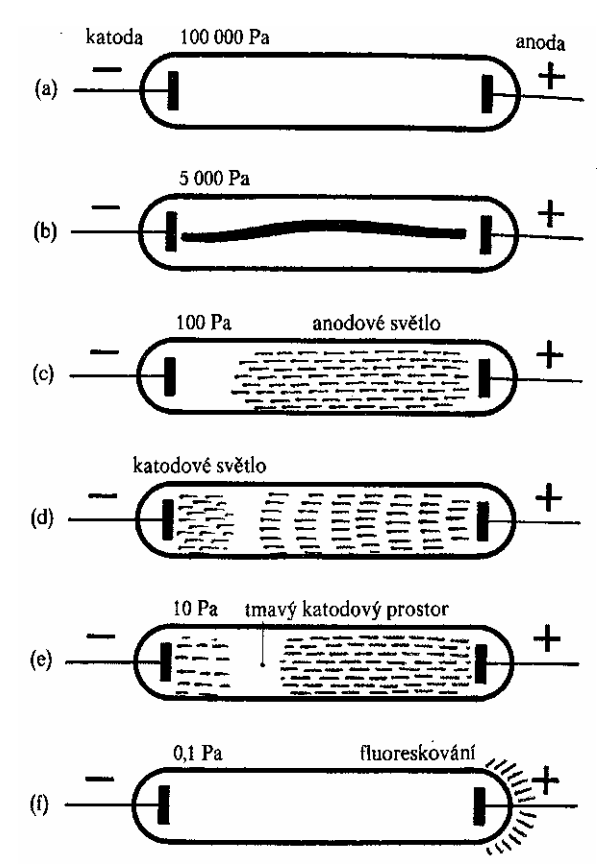
\includegraphics[width = 170 pt]{Figure/01/katody.png}
\caption[Efekty v katodové trubici při snižování tlaku.]{Efekty v katodové trubici při snižování tlaku. Převzato z~\cite{Plyny}}
\label{01katody}
\end{figure}

Jelikož bylo toto záření v průběhu let hojně zkoumáno, byly také pozorovány tyto jeho specifické vlastnosti:
\begin{itemize}
\item nepůsobí-li na něj vnější elektrické nebo magnetické pole, šíří se rovnoměrně přímočaře,
\item je vychylováno elektrickým a magnetickým polem,
\item interaguje s látkou, způsobuje zahřátí, světélkování a chemické procesy,
\item proniká tenkými vrstvami a rozptyluje se,
\item při dopadu na kovy s vysokou relativní atomovou hmotností vyvolává RTG záření,
\item má mechanické účinky (pokus s roztočením Crooksova mlýnku).
\end{itemize}

Elektronový svazek se využívá v obrazovkách osciloskopu a dříve také ve starých televizích a monitorech. V těchto zařízeních je elektronový svazek vychylován elektrickým nebo magnetickým polem. Na stejném principu funguje i náš experiment.

\section{Elektrický proud ve vakuu}
Vakuem obecně elektrický proud neprochází, jelikož neobsahuje nabité částice. Aby mohl proud vakuem procházet, je nutné uvolnit nositele náboje na elektrodách.

Jak už bylo zmíněno výše, tok elektronů ve vakuu má velké praktické využití a je důležitý i pro náš experiment. Jeho široké využití je založeno na těchto vlastnostech elektronů:

\begin{itemize}
\item mají nepatrnou hmotnost, proto mají ze všech částic největší měrný náboj, takže i ve slabých elektrických nebo magnetických polích získávají velkou rychlost na poměrně krátké dráze,
\item přenos náboje u nich prakticky není spojen s přenosem látky,
\item lze je snadno získat mnoha způsoby uvolňováním z kovů.
\end{itemize}

Uvolňování elektronů z kovů probíhá zahřátím vodiče na vysokou teplotu, čímž získají některé elektrony, které se za normálních okolností ve vodiči neuspořádaně pohybují, dostatečnou rychlost, aby překonaly vnitřní přitažlivé síly a vylétly z vodiče ven. Tomuto jevu se říká termoemise. Při termoemisi se původně neutrální vodič stává kladně nabitým, což způsobuje následné přitahování elektronů zpět na povrch vodiče, čímž vzniká tzv. elektronový mrak. 

%princip změny polohy?
%
%\begin{figure}[htbp!]
%\centering
%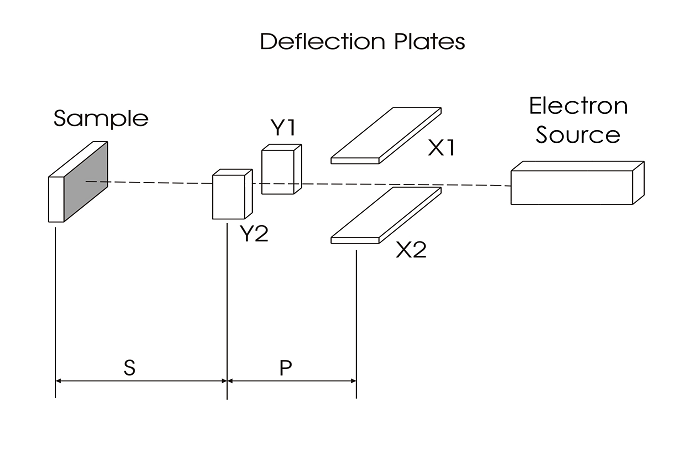
\includegraphics[width = 170 pt]{Figure/04/schema2.png}
%\caption{. Převzato z~\cite{Manual}}
%\label{04schema2}
%\end{figure}


\newpage
\chapter{Elektrické výboje}
\par Při přípravě elektronového svazku jsme se snažili, aby byl dostatečně energetický pro dosažení prahu detekce použitého detektoru. Proto jsme cílili na dosažení elektronového svazku o energii zhruba 80 keV. Urychlení jsme prováděli pomocí rozdílu elektrického potenciálu na měděných elektrodách použitím zdrojů kladných pólů napětí. 
\par K dosažení zamýšlené energie elektronového svazku jsme použili zdroj vysokého napětí (HV) s rozsahem až do 100 kV a dva zdroje o maximálním rozsahu 5 kV. Experiment jsme prováděli ve vakuové komoře. U průchodky do vakuové komory jsme však nebyli schopni elektrody od sebe izolovat z důvodu špatné přístupnosti, takže jak z vnitřní, tak z vnější strany byla vzdálenost mezi elektrodami menší než jeden centimetr. V tomto místě hrozilo, že dojde k elektrickému výboji.

\section{Teorie elektrického výboje}
\par Základním dělením elektrických výbojů je dělení na samostatné a nesamostatné \cite{kracik}. Nesamostatné výboje jsou vázány na vnější (tzv. ionizační) činidlo, bez kterého nemohou probíhat. Ionizačním činidlem mohou být například elektrony vystupující ze žhavené katody nebo ozařování výbojového prostoru rentgenovými paprsky. Pokud se výboj může udržet, i když ionizační činidlo nepůsobí, nazýváme ho samostatným. Takovými výboji jsou výboje temné, doutnavé, obloukové, jiskrové, vysokofrekvenční a koróny. Dále rozebereme doutnavé a jiskrové výboje \cite{kracik}.

\subsection{Samostatné výboje}
\par Teorie samostatného výboje vznikla z rozšíření teorie nesamostatného výboje. Teorie nesamostatných výbojů je založena na myšlence Townsendových lavin, kdy žhavená katoda produkuje stálý počet elektronů za jednotku času, které dále ionizují částice plynu mezi elektrodami a produkují se laviny. U samostatného výboje již uvažujeme dostatečně vysoké napětí mezi elektrodami, že ionizační činidlo není zapotřebí a výboj probíhá pomocí vysokého počtu ionizací nárazem.
\par Minimální napětí na elektrodách, které je potřeba ke vzniku výboje $U_z$, tj. zápalné napětí samostatného výboje, lze podle Townsenda vypočítat jako \cite{kracik}

\begin{equation} 
U_z=A \frac{pd}{\ln \Big[ B \frac{pd}{\ln \big( 1+ \frac{1}{\eta_+} \big)} \Big]} \quad \text{,}
\label{eq:paschen}
\end{equation}

kde $A=BU_i$ a $U_i$ je ionizační napětí, $B=\frac{1}{p\lambda_e}$ je počet srážek na jednotku dráhy elektronu při jednotkovém tlaku prostředí, kde $\lambda_e$ je střední volná dráha elektronu, $p$ je tlak, $d$ je vzdálenost elektrod a $\eta_+$ charakterizuje vlastnosti materiálu katody, které ovlivňují pravděpodobnost emise elektronů z katody kladnými ionty (koeficient sekundární emise elektronů). Rovnice \eqref{eq:paschen} je nazývána Paschenovým zákonem. Bylo zjištěno, že konstanty $A$ a $B$ se nemění v oblasti $E/p=450-7500$ $\frac{\text{V}}{\text{kPa} \cdot \text{cm}}$ ($E$ je elektrická intenzita) a jsou rovny $A=2737,5$ $\frac{\text{V}}{\text{kPa} \cdot \text{cm}}$ a $B=112,5$ $\frac{\text{V}}{\text{kPa} \cdot \text{cm}}$ \cite{Husain1982}.
\par Průběh zápalného napětí různých plynů je znázorněn na Obr. \ref{obr:paschen}, specálně pro vzduch na Obr. \ref{obr:paschen_air}. Zápalné napětí $U_z$ nabývá minima v \cite{kracik}

\begin{equation}
(pd)_{min}=\frac{2,781}{B} \ln \Big( 1+ \frac{1}{\eta_+} \Big) \quad \text{.}
\end{equation}


\begin{figure}[h!]
\centering
\begin{minipage}[c]{200pt}
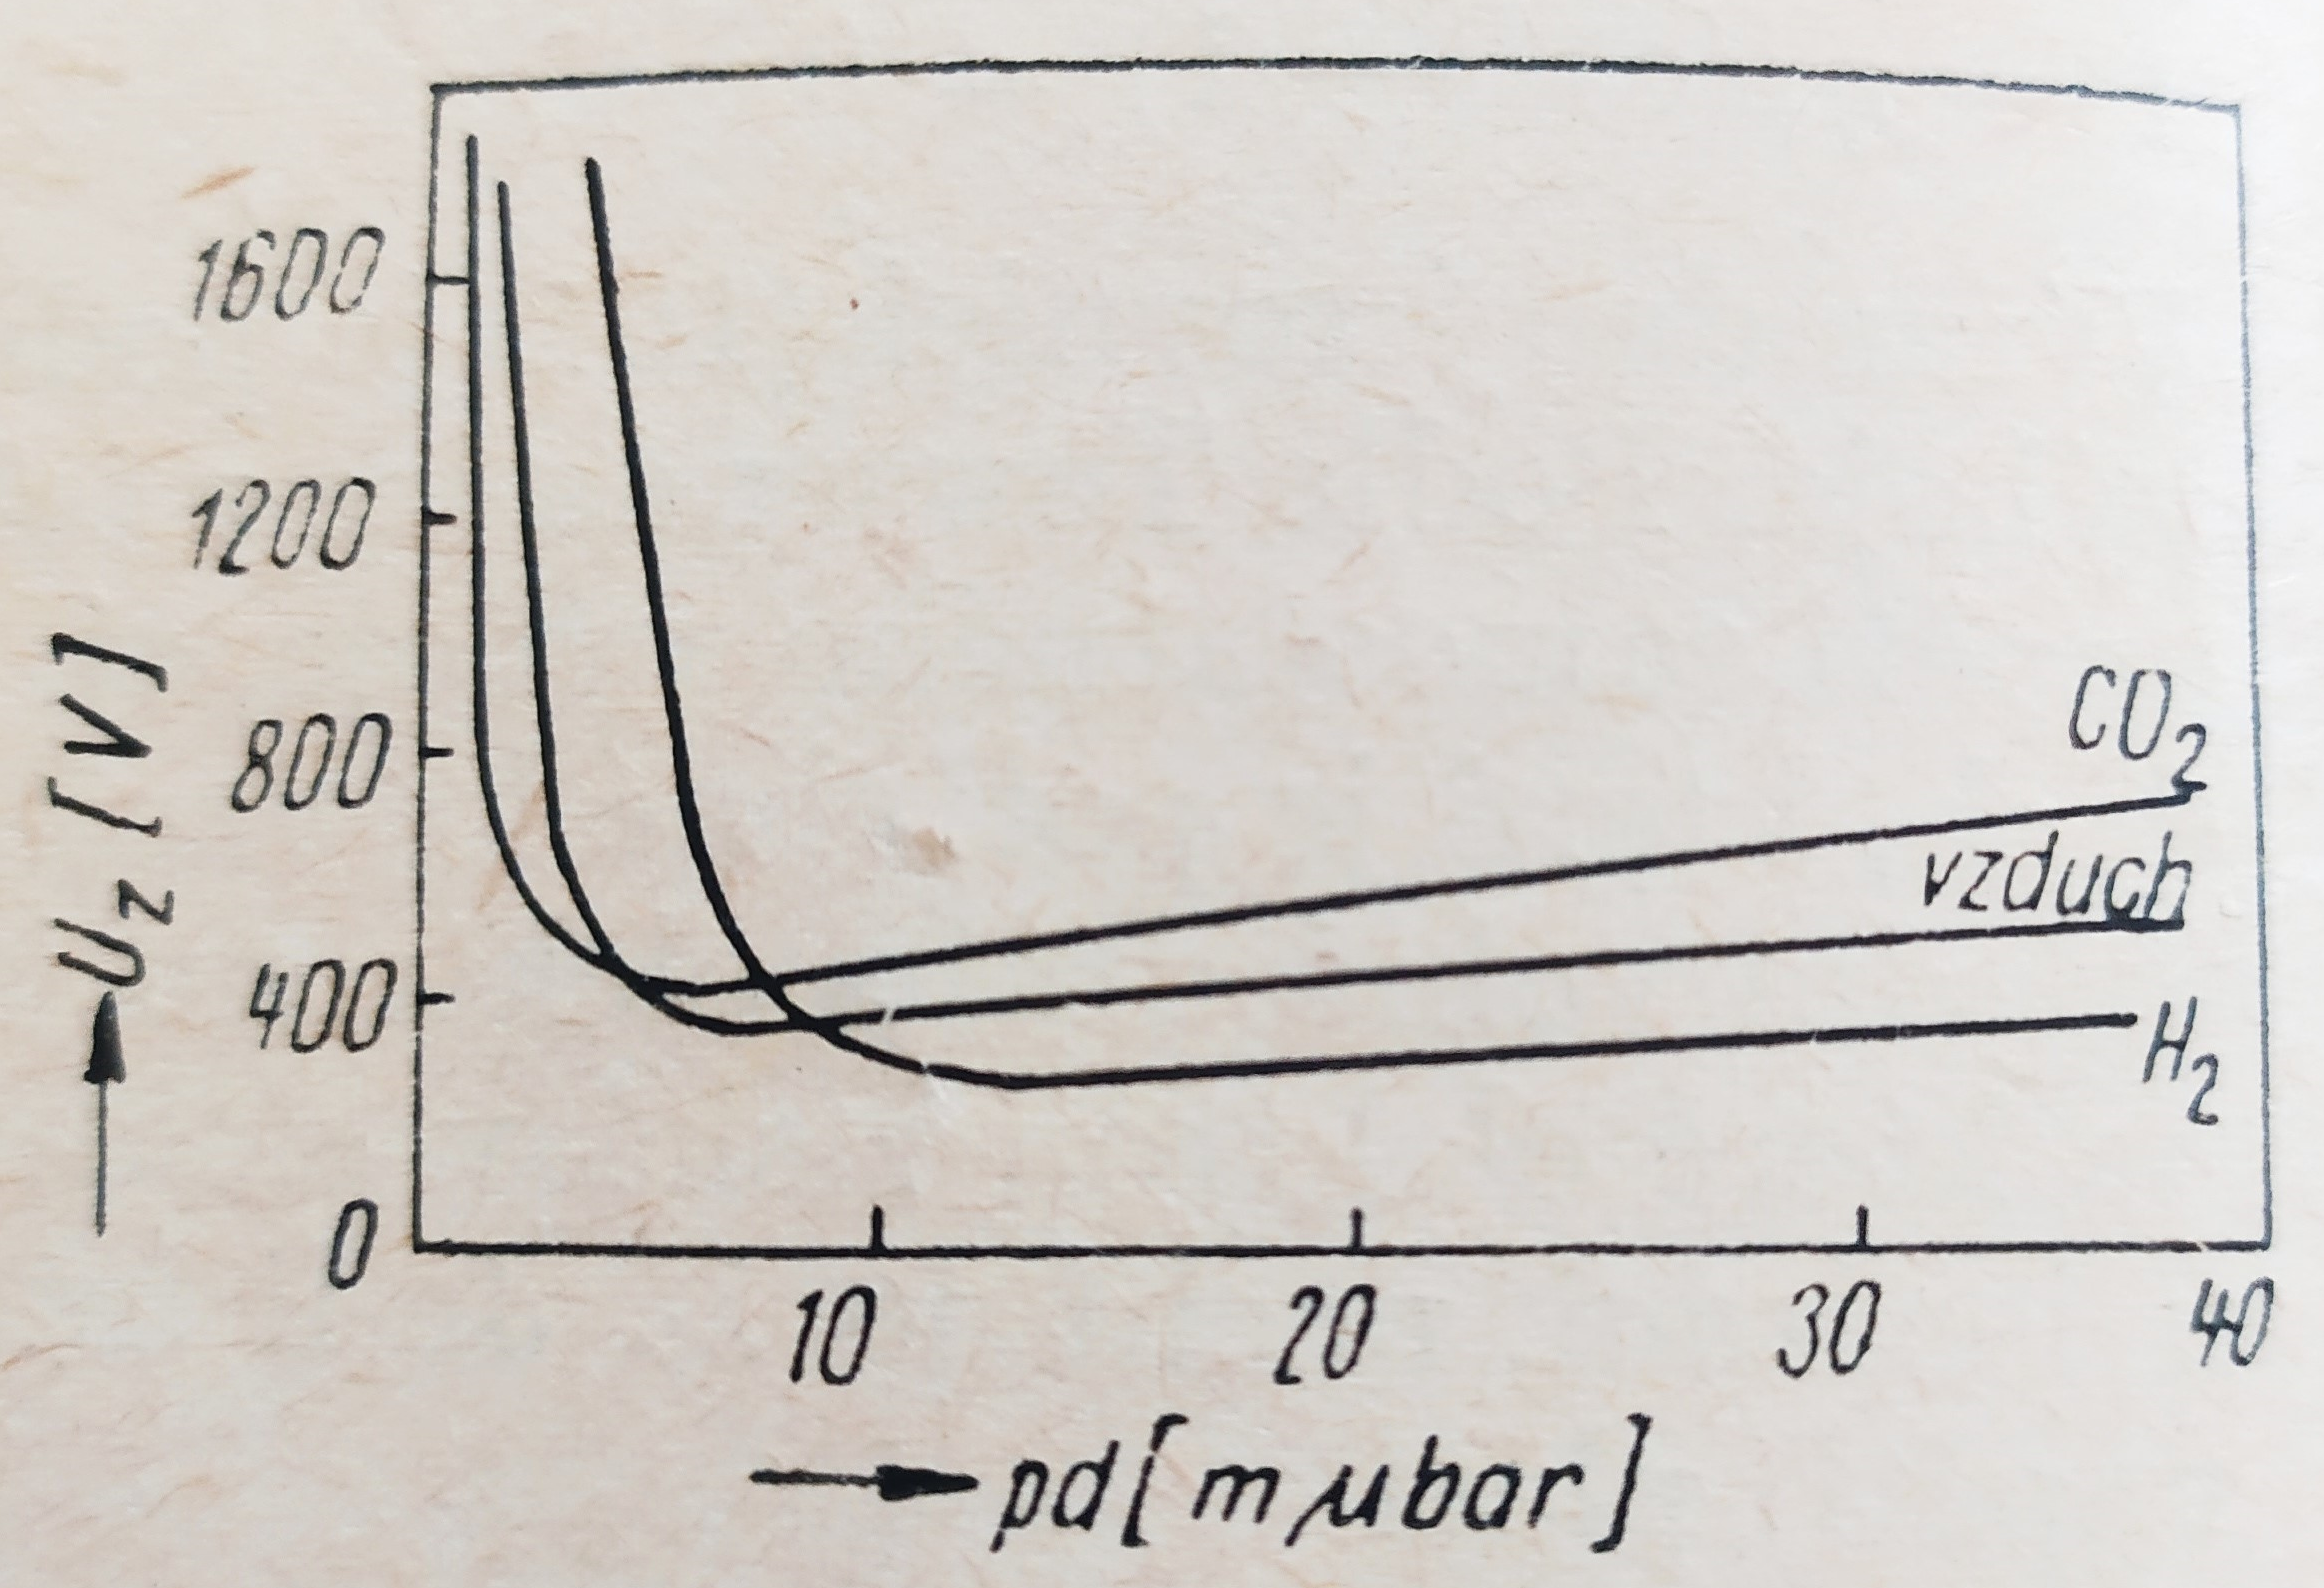
\includegraphics[width=\textwidth]{Figure/02/paschen.png}
\end{minipage}
\begin{minipage}[c]{200pt}
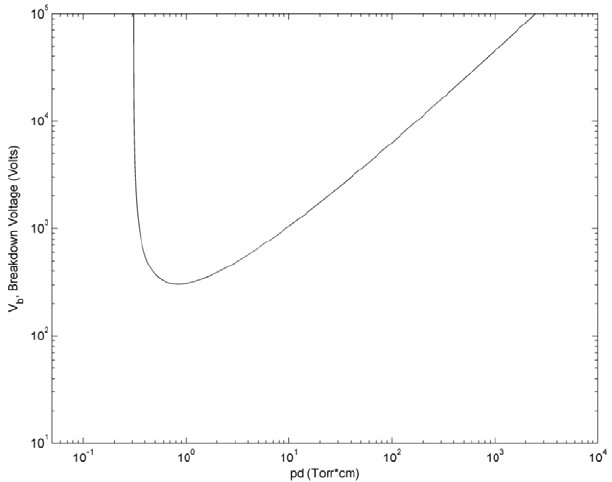
\includegraphics[width=\textwidth]{Figure/02/paschen_air.png}
\end{minipage}
\\
\begin{minipage}[c]{200pt}
\caption{Zápalné napětí různých plynů \cite{kracik}. (1~$\mu$bar = 0,1 Pa)}
\label{obr:paschen}
\end{minipage}
\begin{minipage}[c]{5pt}
\end{minipage}
\begin{minipage}[c]{200pt}
\caption{Paschenova křivka pro vzduch z roku 2011 \cite{Martins2011}. (Torr$\cdot$cm = 133 Pa$\cdot$cm)}
\label{obr:paschen_air}
\end{minipage}
\end{figure}

\subsubsection{Doutnavý výboj}
\par Přechod od nesamostatného výboje k samostatnému je doprovázeno vzrůstem proudu a světélkováním plynu. Pro doutnavý výboj jsou charakterizující světélkující oblasti především u anody, kde dochází k nejvíce srážkám elektronů s molekulami plynu \cite{kracik}. V závislosti na rozložení prostorových nábojů se průběh potenciálu mezi katodou a anodou deformuje a světélkující oblasti se nacházejí i dále od anody. Rozložení prostorových nábojů se mění i s tlakem \cite{edu-techmania}. Na Obr. \ref{obr:doutnavy} je znázorněn doutnavý výboj ve vzduchu při tlaku 100 Pa.

\subsubsection{Jiskrový výboj}
\par Jiskrový výboj je nestabilní a nestacionární forma samostatného výboje, která nevyžaduje působení ionizačního činidla \cite{kracik}. Má vzhled jasně svítících větvících se kanálů o vysoké teplotě a v plynu je doprovázen akustickými jevy. Přestože se při jiskrových výbojích uplatňuje jiný princip vzniku než při výboji lavinovém, tzv. kanálový mechanismus, platí pro ně Paschenův zákon \eqref{eq:paschen} \cite{kracik}. Jelikož se součinitel $\eta_+$ vyskytuje v Paschenově zákoně ve tvaru $\ln \ln \eta_+$, materiál katody nemá vliv na velikost $U_z$ \cite{kracik}. Zápalné napětí je nazýváno napětím průrazu a u vzduchu činí toto průrazné napětí při normání teplotě a tlaku 3 MV/m = 30 kV/cm \cite{tipler1987}.

%napočítat hodnoty napětí pro průraz s tim, že eta dáme třeba 40 podle 
%https://arxiv.org/ftp/arxiv/papers/1302/1302.2333.pdf 
%https://arxiv.org/ftp/arxiv/papers/1302/1302.2334.pdf
% dále doutnavý a jiskrový výboj a pak popis naší aparatury a co jsme pozorovali - to fialový a pak blesk, jak jsme to vyřešili (izolace nefungovala, přendání, nižší napětí)


\begin{figure}[h!]
\centering
\begin{minipage}[c]{200pt}
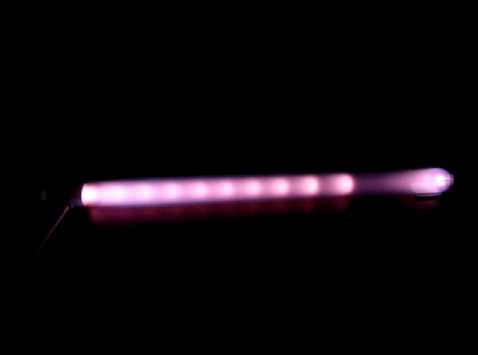
\includegraphics[width=\textwidth]{Figure/02/doutnavy.png}
\end{minipage}
\begin{minipage}[c]{200pt}
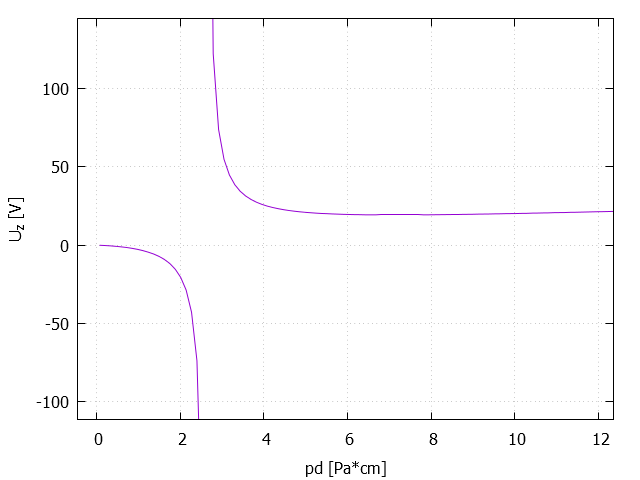
\includegraphics[width=\textwidth]{Figure/02/paschen_moje.png}
\end{minipage}
\\
\begin{minipage}[c]{200pt}
\caption{Ekvipotenciální plochy v doutnavém výboji při 100 Pa \cite{edu-techmania}.  }
\label{obr:doutnavy}
\end{minipage}
\begin{minipage}[c]{5pt}
\end{minipage}
\begin{minipage}[c]{200pt}
\caption{ Funkce f(x) je vykreslená Paschenova křivka \eqref{eq:paschen} pro hodnoty $A=2737,5$ $\frac{\text{V}}{\text{kPa} \cdot \text{cm}}$, $B=112,5$ $\frac{\text{V}}{\text{kPa} \cdot \text{cm}}$ a $\eta_+=3$.}
\label{obr:paschen_moje}
\end{minipage}
\end{figure}


\section{Přivedení vodičů k elektrodám}
\par K elektrodám, které sloužily jak pro urychlení, tak i k fokusaci elektronového svazku, jsme přiváděli jeden vodič s napětím vyšším než 20 kV a dva s napětím do 5 kV. Nejprve jsme se pokoušeli použít jedinou průchodku, u které byly všechny sousední vodiče vzdáleny méně než jeden centimetr. Podle teorie by k výboji na vzduchu mělo docházet při zhruba 20 kV/0,7 cm, což nebylo pro naše účely nedostatečné a vysoké napětí jsme přiváděli samostatnou průchodkou.
% My jsme však nebyli schopni získat z vysokonapěťového zdroje více než 5 kV pravděpodobně kvůli neúmyslnému uzemnění v jiném místě. Naším cílem bylo navíc vést vodičem více než 20 kV, čímž bychom překročili dielektrickou pevnost vzduchu. Vysoké napětí jsme tedy přiváděli samostatnou průchodkou a původní průchodkou jsme vedli pouze vodiče do 5 kV. 
\par Samostatná průchodka však nebyla uzpůsobena k vedení vysokého napětí a opět byl vodič vzdálen zhruba 1 cm od uzemněné vakuové komory. I přes naši snahu nechráněné části průchodky co nejvíce izolovat vulkanickou páskou jsme při překročení napětí 30 kV na vzduchu výboje pozorovali. Vysokonapěťovou keramicky izolovanou průchodku jsme bohužel k dispozici neměli.
\par Uvnitř komory byly jednotlivé elektrody vzdáleny od sebe navzájem a od uzemněné komory také přibližně jeden centimetr. Abychom mohli použít výpočet pomocí Paschenova zákona \eqref{eq:paschen}, je potřeba, aby podíl elektrické intenzity $E$ a tlaku $p$ byl v rozmezí $E/p=450-7500$ $\frac{\text{V}}{\text{kPa} \cdot \text{cm}}$. Námi cílený tlak byl ideálně co nejmenší, abych se náš elektronový svazek nerozptyloval na molekulách vzduchu, tedy $10^{-2}-10^{-4}$ Pa. Pro napětí $U$ v řádu kilovoltů však ze vztahu $E=U/d$ dostáváme pro $d=1$ cm $E/p \sim 10^{9}$ $\frac{\text{V}}{\text{kPa} \cdot \text{cm}}$. I kdybychom se rozhodli toto omezení nerespektovat, zjistíme, že z Paschenova zákona dostaneme pro námi zamýšlené hodnoty $p=10^{-3}$ Pa a $d=1$ cm nesmyslný výsledek $U_z<0$ \footnote{Použili jsme $A=2737,5$ $\frac{\text{V}}{\text{kPa} \cdot \text{cm}}$, $B=112,5$ $\frac{\text{V}}{\text{kPa} \cdot \text{cm}}$ a $\eta_+=3$ \cite{Bozhko}. Volba jiného $\eta_+$ v rozmezí $\eta_+=2-100$ výsledek nemění.}, jelikož má závislost \eqref{eq:paschen} průběh hyberboly (Obr. \ref{obr:paschen_moje}).
%což potvrzuje neaplikovatelnost \eqref{eq:paschen}. Jelikož má závislost \eqref{eq:paschen} průběh hyberboly (Obr. \ref{obr:paschen_moje}), je chybné se domnívat, že pro námi dosahované oblasti $10^{-4}$ Pa$\cdot$cm $\sim 8\cdot 10^{-7}$ Torr$\cdot$cm by $U_z$ šlo do nekonečna (Obr. \ref{obr:paschen_air}). 
Proto jsme neexistenci výboje v komoře odhadovali pouze na základě úvahy, že při dosaženém nízkém tlaku nebude pro výboj k dispozici dostatečný počet ionizovatelných molekul.



\section{Pozorování a diskuse}
\par Při prvních zkouškách jsme dosahovali tlaku zhruba 100 Pa a při použitém napětí 3 kV jsme pozorovali fialový doutnavý výboj (Obr. \ref{obr:fialovy_vyboj}). Naše pozorování se shoduje s očekáváním z Obr. \ref{obr:doutnavy}. Současně jsme však nepozorovali žádný signál elektronů na stínítku. Použité wolframové vlákno pravděpodobně nebylo vhodným zdrojem elektronů. 
% jako zdroje elektronů, které nám buď nedodávalo dostatečný počet elektronů, anebo jsme elektrony nebyli schopni od vlákna urychlit ke stínítku kvůli nevhodnému sestavení aparatury. 
\par Další pokusy jsme prováděli při tlaku přibližně 10$^{-2}$ Pa \footnote{Jelikož se nám ke konci semestru porouchal tlakoměr, dosažený tlak řádu 10$^{-2}$ Pa jsme odhadovali na základě alespoň třídenního čerpání vakuové komory turbomolekulární vývěvou. }. Při nich jsme již nepozorovali doutnavý výboj, ale při dosažení napětí 20 kV na urychlovací elektrodě jsme v komoře pozorovali výboje doprovázené zelenými záblesky. Pravděpodobně se jednalo o elektrony vzniklé při výboji, které dopadly na instalované fluorescenční stínítko, jelikož jsme stejné zelené světlo pozorovali na stínítku při dopadu elektronů z funkčního elektronového děla. Tyto výboje se v závislosti na použitém napětí pravidelně opakovaly a se zvyšujícím se napětím se časové intervaly mezi nimi zkracovaly. Do komory jsme viděli malým průzorem a záblesk vždy osvítil celou komoru, takže jsme ani nebyli schopni určit, kde k výbojům dochází. Výboje jsme pozorovali i v případě, kdy jsme zapojili pouze jednu elektrodu s nejvyšším urychlovacím napětím, domníváme se proto, že docházelo k výboji do komory v místě, kde byla vzdálenost elektrody od komory nejkratší. Při jednom výboji jsme dokonce pozorovali jasný jiskrový výboj (Obr. \ref{obr:jiskra}), ovšem na jiném místě.

\begin{figure}[h!]
\centering
\begin{minipage}[c]{200pt}
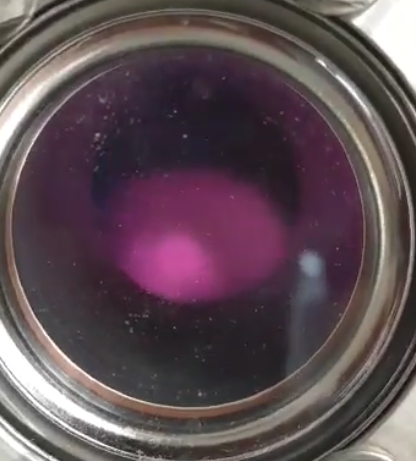
\includegraphics[width=\textwidth]{Figure/02/fialovy_vyboj.png}
\end{minipage}
\begin{minipage}[c]{200pt}
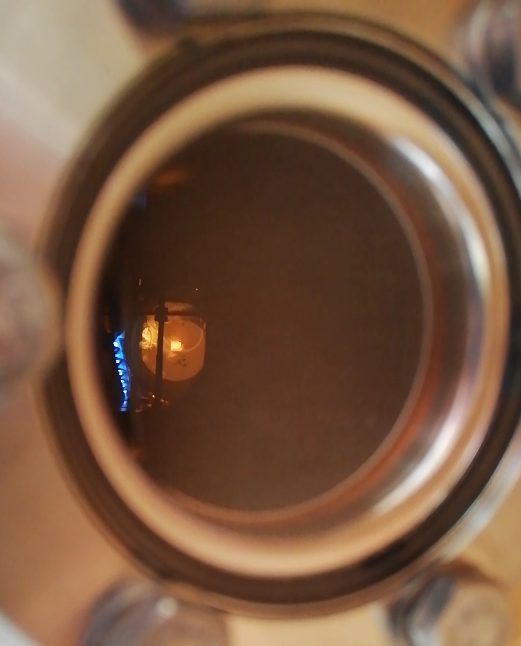
\includegraphics[width=\textwidth]{Figure/02/jiskra.png}
\end{minipage}
\\
\begin{minipage}[c]{200pt}
\caption{Pozorovaný fialový doutnavý výboj při tlaku zhruba 100 Pa.  }
\label{obr:fialovy_vyboj}
\end{minipage}
\begin{minipage}[c]{5pt}
\end{minipage}
\begin{minipage}[c]{200pt}
\caption{Pozorovaný jiskrový výboj při tlaku zhruba $10^{-2}$ Pa.}
\label{obr:jiskra}
\end{minipage}
\end{figure}


\par Při použití napětí vyššího než 30 kV jsme pozorovali výboje již u průchodky vysokého napětí z vnějšku komory na vzduchu. Výbojům jsme se snažili zabránit zvýšenou izolací vodičů vulkanickou páskou a plastovou ohebnou trubkou. Neúspěšně. Pro měření s detektorem dodaným od druhé skupiny jsme proto volili pouze urychlovací napětí do 18 kV, aby detektor výboje nepoškodily, což zkomplikovalo měření, protože jsme nedosáhli cílené energie elektronů 80 keV.
\par Navzdory našemu očekávání docházelo k výbojům ve vyčerpané vakuové komoře při nižším napětí než na vzduchu. Pro tento jev nemáme uspokojivé vysvětlení. Navíc při tlacích menších než 1,3 Pa by nemělo docházet k žádným elektrickým výbojům při jakémkoli napětí \cite{ellion}. Výboje by snad odstranilo použití keramické vysokonapěťové průchodky.

%výboje když jsme zapojili jen HV a nic jiného, výboje při 18 kV, víc jsme nepoužívali, abychom nezničili detektor



\section{Závěr}
\par K urychlení elektronů jsme se na elektrody do vakuové komory snažili přivést napětí řádu 5 kV a vysoké napětí řádu 80 kV. K vedení vysokého napětí jsme použili samostatnou průchodu, která však stejně jako původně použitá nevyhovovala podmínkám vedení vysokého napětí a při napětí vyšším než 18 kV uvnitř komory a napětí vyšším než 30 kV z vnějšku komory probíjela. Tyto hodnoty jsme proto nepřekračovali. Průchodka pro vedení napětí řádu 5 kV byla dostatečná a výboje jsme nepozorovali.
\par Navrhovaným řešením výbojů je použití keramické průchodky uzpůsobené k vedení vysokého napětí.
\newpage

\chapter{Architektura elektronového děla}
Nejdříve se zaměříme na možné praktické zdroje volných elektronů. Pro potřeby elektronového děla se využívá fotoelektrického jevu -- fotoemise, poté tzv. studené emise elektronů z látky indukované silným elektrickým pole a nejčastěji využívaná termoemise elektronů. Právě termoemise, jako zvolená metoda pro generování volných elektronů, bude důkladněji rozebrána. Dále si představíme námi použitá elektronová děla: vlastní soustavu využívající termoemise z wolframového vlákna se čtyřmi elektrodami a finální setup průmyslového elektronové děla s přidanou soustavou čtyřech elektrod.
\section{Zdroje volných elektronů}
Obecně je nutné dodat elektronům v látce, většinou kovu, dostatečnou energii k překonání vazebných sil s atomy látky, čímž se uvolní do prostoru (uvažujme vakuum). Dochází i k tunelovému jevu, jako je tomu u studené emise. Uvolněné elektrony mohou být následně urychleny elektrostatickým polem.
\subsection{Fotoemise} Tato emise elektronů z látky je způsobena fotoelektrickým jevem, tj. interakcí vázaných elektronů v atomech s externími přilétajícími fotony. Využívá se záporně nabité katody, která je ozařována z vnějšího zdroje fotony o dostatečné frekvenci $f$, resp. energii $hf$ k uvolnění vázaných elektronů v látce. Uvolněné elektrony mají poté ze známého vztahu maximální kinetickou energii rovnu $E_{kin}=hf-W$, kde $W$ je z \textit{work function} -- minimální energie nutná pro uvolnění elektronu z látky. Hovoříme o maximální kinetické energii z důvodu možné realizace Comptonova rozptylu, kdy poté foton nezanechá všechnu svou energii v jedné interakci s elektronem, ale po interakci se šíří dále s nižší frekvencí, resp. energií. Takový zdroj elektronů má poté nediskrétní spektrum, avšak vzhledem k mnohem větším škálám následného urychlení lze tento rozdíl zanedbat. 
\subsection{Studená emise} Název této emise elektronů je dán, kvůli kontrastu s termoemisí. Uvažujme pevnou látku (kov) a přiveďme napěťový spád mezi něj a okolní prostor (vakuum), tak aby emitující materiál byl katodou jako na Obr. \ref{CFEpotent}. Můžeme vidět \textit{field-free potential barrier}, kdy tento potenciál případu bez externího pole zabraňuje elektronům pod Fermiho hladinou opouštět daný materiál a k jeho překonání je potřeba výstupní práce $W$. Přidáme-li však napěťový spád, tím potenciál -- \textit{potential of the applied field}, tak pro uvolnění elektronů z látky je nutné efektivně překonat superponovaný potenciál vyznačený na Obr. \ref{CFEpotent} nepřerušovanou černou čarou. Tato vzniklá potenciálová bariéra může být statisticky elektronem protunelována a daný elektron je poté ve volném prostoru mimo látku a urychlován spádem napětí externího pole. Je nutné dodat, že jak bylo teoreticky předpovězeno, tak úzký hrot látky emituje elektrony snáze, a proto se využívá hrotů jako na Obr. \ref{CFE} vpravo. Celého principu lze například využít u elektronových tunelových mikroskopů, kdy namísto tunelování elektronů do volného prostoru, tunelují do zkoumaného vzorku v určitém počtu úměrném vzdálenosti mezi emitujícím hrotem a povrchem vzorku. 

\begin{figure}[htbp!]
	\centering
	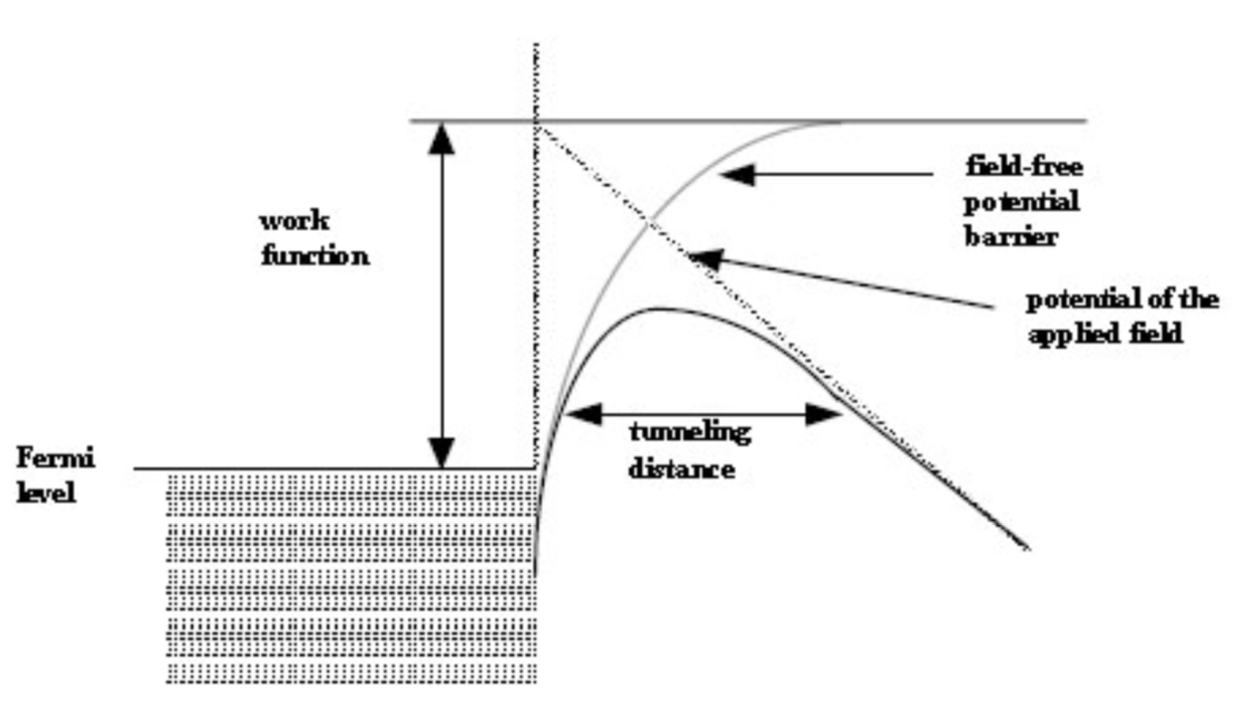
\includegraphics[width = 350 pt]{CFEpotent.png}
	\caption{Průběh potenciálů v blízkosti rozhraní emitující látky a vakua. Převzato z~\cite{coldems}.}
	\label{CFEpotent}
\end{figure}

\begin{figure}[htbp!]
	\centering
	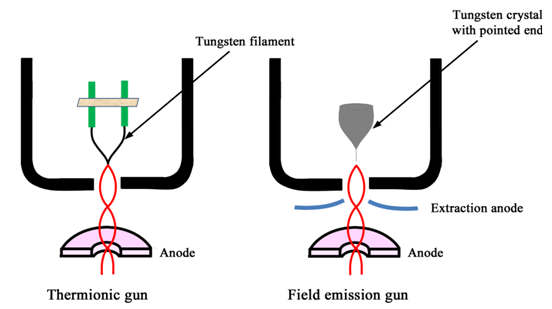
\includegraphics[width = 350 pt]{CFE.png}
	\caption{Schémata možné realizace zdroje elektronů. Vlevo: termoemise elektronů z wolframového vlákna. Vpravo: studená emise elektronů z hrotu krystalu wolframu. Převzato z~\cite{zdrojel}.}
	\label{CFE}
\end{figure}

\subsection{Termoemise}
K uvolnění elektronů lze využít i tepelné energie $kT$, kde $k$ je Boltzmanova konstanta a $T$ je termodynamická teplota. Tato tepelná energie, představující střední kinetickou energii elektronů v látce, může být srovnatelná s výstupní prací elektronů z látky $W$, v tom případě elektrony s dostatečnou energií opouští povrch látky do prostoru. Hustota emisního proudu elektronů $J$ se řídí dle Richardson-Duschmanova zákona:
\begin{equation}
	J=BT^2\exp(-\frac{W}{kT}),
	\label{RDlaw}
\end{equation}
kde $B$ je charakteristická konstanta každého materiálu. 
\begin{figure}[htbp!]
	\centering
	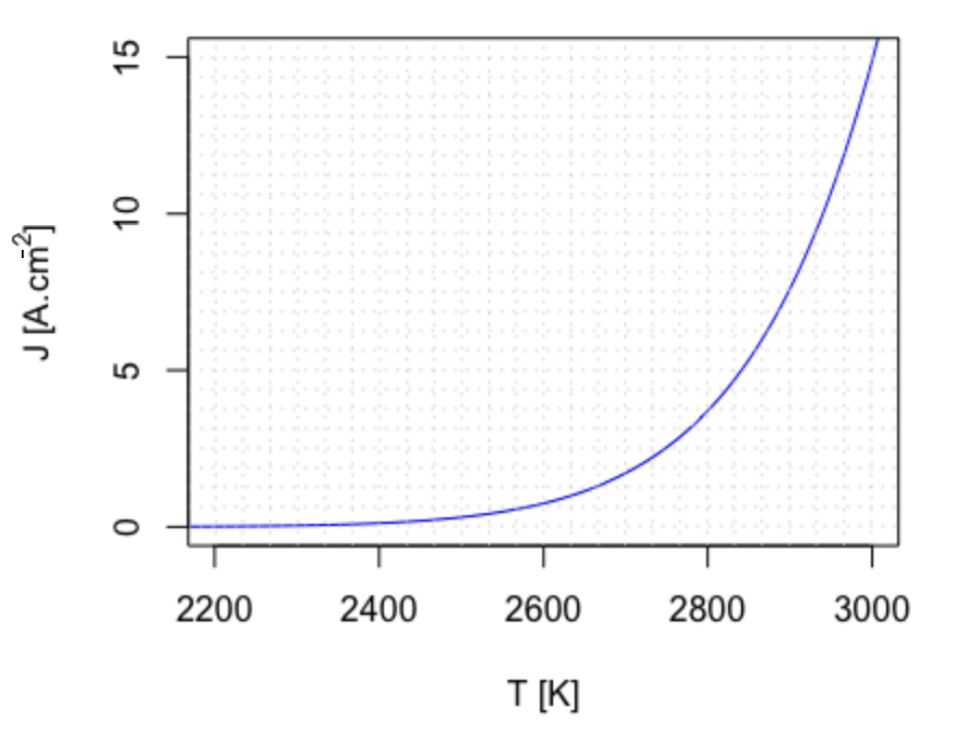
\includegraphics[width = 350 pt]{WolframGraf.png}
	\caption{Závislost emisního proudu $J$ z wolframu na jeho teplotě $T$ dle Richardson-Duschmanova vztahu (\ref{RDlaw}), pro wolfram $W=4,54$ eV a $B=60$ Acm\textsuperscript{-2}K\textsuperscript{2} ~\cite{zdrojwolf}.}
	\label{WolframGraf}
\end{figure}
\par Kvůli tepelné odolnosti a malé výstupní práci $W=4,54$ eV ~\cite{zdrojwolf} se jako emisního materiálu využívá zejména wolframu s možnými přiměsmi pro snížení výstupní práce. Navíc wolfram jako vodič může být zahříván pomocí ohmického ohřevu a být stálý i při teplotách okolo 3000 K. Jak lze vidět na Obr. \ref{WolframGraf}, kde je vyobrazen Richardson-Duschmanův vztah pro wolfram s $B=60$ Acm\textsuperscript{-2}K\textsuperscript{2} ~\cite{zdrojwolf}, při teplotách nad 2600 K z wolframu vyletuje vysoký proud elektronů. 
\par Musíme však vzít v potaz povrch námi použitého wolframového vlákna. Využili jsme wolframového vlákna stočeného do šroubovice se zruba $n=70$ závity, výška šroubovice je $h_s=0,5$ cm, průměr samotného vlákna byl $r=h_s/100$ cm a průměr podstavy opisovaného válce šroubovicí zhruba $d=6r$ ($h_s$ odpovídá výšce celého válce). Odsud lze vypočíst výšku válce potřebnou pro jednu otočku (\textit{revolution}) šroubovice jako $h_{rev}=h_s/n$, poté platí úvaha dle Obr. \ref{HevixUnWrap}, že rozvineme-li plášť tohoto malého válce s jednou otočkou šroubovice, tak dostaneme obdélník, jehož úhlopříčka je délka šroubovice na jednu otočku $l_{rev}$ a strany obdélníku jsou rovny $h_{rev}$ a $\pi d$, proto 
\begin{equation}
l_{rev}=\sqrt{h_{rev}^2+(\pi d)^2},
\end{equation}
odsud $l_{rev}\simeq 0,09$ cm. Jelikož otoček jsme měli právě $n=70$ a délka drátu na jednu otočku je $l_{rev}$, je celková délka rozbaleného drátu $l=nl_{rev}\simeq 6,6$ cm. Nyní lze již snadno vypočíst povrch šroubovice jako $S=2\pi r l$ s výsledkem $S=0,2$ cm\textsuperscript{2}. Odsud předpokládáme-li teplotu wolframového vlákna okolo 2600 K, což odpovída emitujícímu proudou okolo $0,625$ Acm\textsuperscript{-2}, tak z našeho vlákna emituje proud o hodnotě zhruba $J=0,129$ A, odpovídající $1,4\times 10^{17}$ elektronům za sekundu.
\begin{figure}[htbp!]
	\centering
	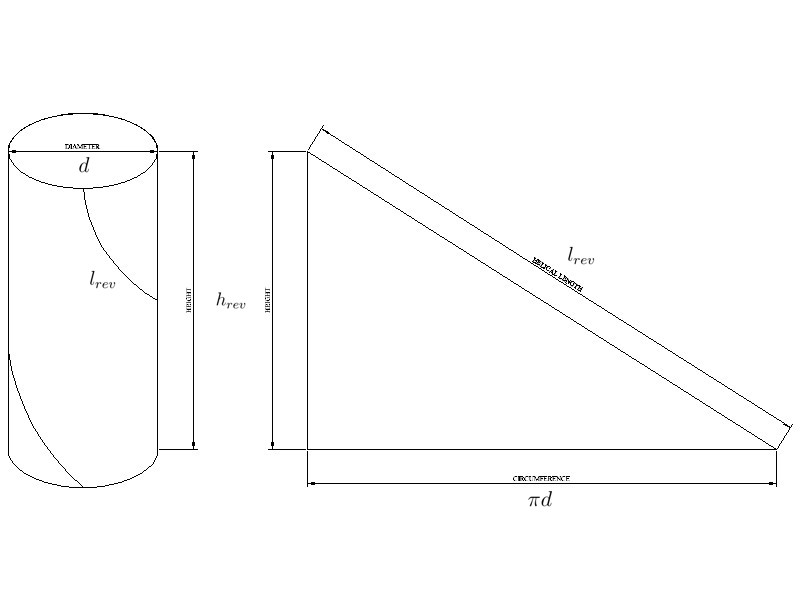
\includegraphics[width = 350 pt]{HevixUnWrap.jpg}
	\caption{Ilustrace odvození délky jednoho závitu šroubovice. Převzato a upraveno z~\cite{curv}.}
	\label{HevixUnWrap}
\end{figure}
\par Zvolili jsme ohmického ohřevu vlákna, kdy jsme připojili zdroj stejnosměrného napětí v rozmezí 0-15 V na svorky wolframového vlákna a do prostoru v okolí emitujícího vlákna umístili válcové anody pro urychlení elektronů a formování svazku, tento urychlovací a fokusační systém bude představen dále a v kapitole \ref{kapFok} a \ref{kapKuba}. V závislosti na napětí se měnilo i spektrum záření z wolframového vlákna, odkud jsme vizuálně odhadli dle modelu záření absolutně černého tělesa, že teplota vlákna přesahuje 2500 K při napětí nad 10 V. 
\par Jinou možností realizace termoemise je umístění ohřevného systému, např. i ohmického drátu, v okolí wolframové plošky či šroubovice, na které je přivedeno záporné napětí, tedy wolframová část je katodou. Kvůli ohřevnému systému dochází k termoemisi na wolframu, která je navíc stimulována napěťovým spádem mezi emitujícím wolframem a okolním prostorem. Tento druh termoemise je zajisté při stejných teplotách efektivnější, než termoemise indukovaná ohmickým ohřevem, protože zde navíc využíváme efektů podobných studené emisi, a to externího potenciálu.
\section{Urychlovací a fokusovací soustava elektrod}
Nyní bylo našim úkolem vytvořit soustavu elektrod sloužící ke správnému formování a urychlení svazku elektronů ze zdroje volných elektronů představených výše. Využívá se katody -- \textit{Wehneltova válce} obepínající zdroj elektronů k cílené prostorové emisi ve směru osy chtěného svazku. Aplikaci Wehneltova válce můžeme vidět na Obr. \ref{CFE}, kde je znázorněn jako část černého válce. Pro správnou volbu jeho geometrie spolu se sérií dalších urychlovacích a fokusovacích elektrod jsme v našem případě zvolili software SIMION (viz kap. \ref{kapKuba}) simulující chování elektronů ve vakuu v přítomnosti rotačně symetrických elektrod. Program dovoluje pro různé zdroje, tím s rozdílně energetickými i prostorově rozloženými elektrony, sestavit z dostupných elektrod teoreticky fungující model elektronového děla o daných vlastnostech svazku.
\par Nebudeme zde představovat první testované elektronové dělo z CRT monitoru, které jsme instalovali do vakuové komory a neúspěšně testovali. Bylo nutné určit napětí, které jsme přiváděli na jednotlivé elektrody, tento postup lze vidět v pololetní zprávě z tohoto projektového praktika -- PPRAK 2018/2019. Neúspěšnost při generaci elektronového svazku byla nejspíše zapříčiněna termoemisiním zdrojem elektronů, kdy bylo wolframové vlákno nejspíše přepálené.
\section{Vlastní elektronové dělo}
Rozhodli jsme se sestavit vlastní elektronové dělo využívající termoemise z wolframového vlákna (halogenová žárovka) a sérii válečkových měděných elektrod, jejichž vliv na formování svazku byl simulován pomocí programu SIMION. Sestavili jsme dvě aparatury využívající termoemise, avšak ani v jednom případě jsme na stínítku s fluorescenční vrstvou neviděli zelené světlo původem z interakce elektronů a atomů fluorescenční látky. Avšak při výbojích na některých z elektrod jsme na stínítku pozorovali záblesky zeleného světla, tím se domníváme, že urychlovací soustava byla funkční a problém byl ve zvoleném zdroji elektronů -- termoemisním wolframu. Z tohoto důvodu jsme vytvořili třetí setup, sestávající se z průmyslového děla, který jsme využili jako zdroj elektronů v rozmezí 0-5 keV spolu se soustavou elektrod mající za cíl kolimace a urychlení svazku elektronů až na energie okolo 20 keV. Vyšších energií elektronů jsme nemohli dosáhnout, neboť maximální napětí, které jsme byli bez probíjení schopni dovést do vakuové komory bylo právě 20 kV. Naším původním cílem bylo získat svazek elektronů o energiích až 80 keV.
\par V programu SketchUp jsme navrhli držáky a kolejnicovou platformu pro pozdější uchycení měděných válečků o průměru 3 cm. Finální verzi vytisknutá na 3D tiskárně PRUSA i3 MK2 pomocí materiálu APL lze vidět na Obr. \ref{SetUp} i v zapojení s elektrodami. Materiál APL vydrží vakuum až 10\textsuperscript{-7} Pa, proto jsme ho využili jako uchycení měděných válečků -- elektrod. Měděné válečky měly různé výšky a dle návrhu z programu SIMION byly rozestaveny tak, aby vzhledem k dostupným zdrojů stejnosměrného napětí bylo možné vytvořit optimální potenciálový spád pro produkci elektronového paprsku. Díky kolejnicového systému upevnění držáků jsme měli zaručenou souosost válečkových elektrod.
\begin{figure}[htbp!]
	\centering
	\includegraphics[width = 350 pt]{SetUp.png}
	\caption{První sestava elektronového děla s držáky z materiálu APL a čtyřmi měděnými elektrodami. Zleva halogenová žárovka a poté následující soustava elektrod.}
	\label{SetUp}
\end{figure}
\subsection{Soustava čtyř elektrod s termoemisí}
První setup z APL držáků a měděných válečků je na Obr. \ref{SetUp}, jak můžeme vidět, žárovka je vně první elektrody. První elektroda tedy není Wehneltovým válcem. Simulaci funkčnosti takové sestavy je možné vidět na Obr. \ref{05simulaceVlastniDelo}, u kterého se nachází i jednotlivá napětí přivedená na elektrody. Toto dělo při zapojení napětí i žhavení wolframového vlákna nejevilo známky produkce elektronového svazku, jelikož jsme nepozorovali excitaci fluorescenčního stínítka. Z toho důvodu jsme přešli k sestavě s vnořením wolframového vlákna do první elektrody, simulace je na Obr. \ref{05simulaceVlastniDeloWehnelt}, první elektroda neplní funkci Wehneltova válce, ale anody. Při tomto setupu jsme na poslední hlavní urychlovací elektrodu připojili kladné napětí 18 kV, jež bylo reálně možné přivést do vakuové komory bez probíjení v okolí propustek. 
\par Při obou nastaveních jsme však nepozorovali interakci elektronového svazku s fluorescenčním stínítkem. Funkčnost fluorescenčního stínítka jsme později ověřili, stejně tak tomu nasvědčovaly zelené záblesky při výbojích v komoře v době zapojení urychlovacích elektrod. Jelikož v tomto případě elektrony doletěly až na stínítko vzdálené od výboje více jak 20 cm, poukazuje to navíc i na funkčnost urychlovacích elektrod. Tedy problém byl nejspíše ve zdroji volných elektronů, tj. v termoemisi z ohmicky ohřívaného wolframového vlákna.
\subsection{Průmyslové elektronové dělo se soustavou elektrod}
Kvůli nefunkčnosti předešlých setupů elektronových děl jsme přistoupili k variantě zprovoznění průmyslového elektronového děla, které jsme využili jako zdroj elektronů, a kdy jsme následně vytvořili přídavnou urychlovací a fokusovací soustavu pro dosažení vyšších energií svazku. Průmyslové elektronové dělo dosahuje energií svazku maximálně 5 keV (kap. \ref{kapTomasT}), což by i pro konverzi elektronů na fotony skrze zlato-měděnou fólii nemuselo být dostatečné. Způsob detekce elektronů pomocí chipu X-CHIP03 a použitá metodika je v kap. \ref{kapMatej} a \ref{kapAnezka}. 
\par Simulace námi použité sestavy pro finální měření na chipu X-CHIP03 je v podkap. \ref{simulaceKuba} spolu s použitými nastaveními napětí na elektrodách. Nejdříve jsme ověřili funkčnost průmyslového elektronového děla pomocí fluorescenčního stínítka a pozorovali vliv na fokusaci svazku na stínítku změnami napětí v soustavě přidaných elektrod.

\newpage
\chapter{Zdroj elektronů, ES40-PS}
\label{kapTomasT}

Z důvodů problémů s nedostatkem elektronů z wolframového vlákna žárovky jsme se rozhodli k použití ES40-PS jako zdroje elektronů. ES40-PS je \textit{Electron Source Power Supply} poskytující svazek elektronů s nastavitelnou energií, hustotou, pozicí a profilem svazku. Dále umožňuje skenování oblasti s nastavitelnou rychlostí skenování. 


Schéma zapojení zdroje elektronů ES40-PS je znázorněno na Obr.~\ref{04schema} vlevo. Zdroj elektronů je upevněn pomocí průchodky do vakuové komory a připojen ke stanici ES40-PS pomocí kabelu s 6-pinovou spojkou. Na Obr.~\ref{04schema} vpravo je zobrazena ukázka ovládacího panelu stanice ES40-PS. 


\begin{figure}[htbp!]
\centering
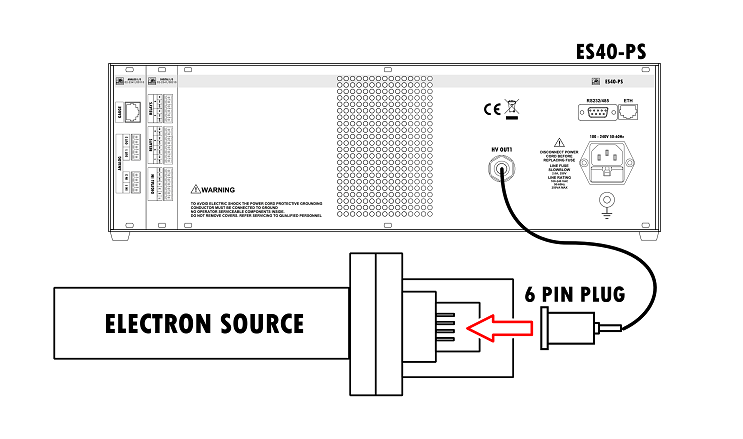
\includegraphics[width = 170 pt]{Figure/04/schema.png}
\hfill
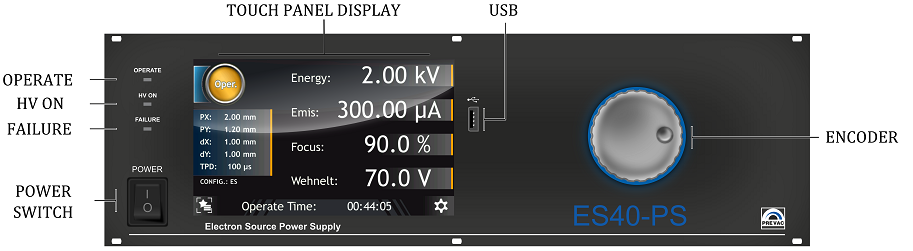
\includegraphics[width = 250 pt]{Figure/04/panel.png}
\caption[Schéma zapojení a ukázka ovládacího panelu stanice ES40-PS]{Vlevo: Schéma zapojení zdroje elektronů ES40-PS. Vpravo: Ukázka předního ovládacího panelu stanice ES40-PS. Převzato z~\cite{Manual}.}
\label{04schema}
\end{figure}

Zdroje elektronů ES40-PS má několik nastavitelných parametrů: 
\begin{itemize}
\item \textbf{Urychlovací napětí} je nastavitelné od 0 kV do 5 kV
\item \textbf{Emisní proud} elektronů je nastavitelný v rozmezí od $0{,}01 \ \mu$A do $300{,}00 \ \mu$A
\item \textbf{Fokusovací napětí} je spojené s urychlovacím a lze nastavit od 60,0 \% do 99,9 \%
\item \textbf{Wehneltovo napětí} od 0 V do 300 V
\end{itemize}
Elektrony vychází ze zahřívání wolframové katody, z tohoto důvodu se může objevit zpráva "Current Limit", kdy je zapotřebí více času ke stabilizaci emisního proudu. 

Zmíněné hodnoty je možné nastavit na úvodní obrazovce ovládacího panelu viz Obr.~\ref{04display}. Po kliknutí na zmenšený seznam hodnot nacházející se v levé části se display přepne do druhé polohy, kde je možné nastavit následující hodnoty:
\begin{itemize}
\item \textbf{Horizontální výchylka} PX je nastavitelná v rozmezí od $-5{,}00$ mm do $5{,}00$ mm 
\item \textbf{Vertikální výchylka} PY je nastavitelná v rozmezí od $-5{,}00$ mm do $5{,}00$ mm 
\item \textbf{Horizontální rozsah skenu} dX je nastavitelný v rozmezí od $0{,}00$ mm do $10{,}00$ mm
\item \textbf{Vertikální rozsah skenu} dY je nastavitelný v rozmezí od $0{,}00$ mm do $10{,}00$ mm
\item \textbf{TPD hodnota} (\textit{time per dot}) je nastavitelný v rozmezí od $20 \ \mu$s  do $30$ ms
\end{itemize}

Všechny výše uvedené parametry byly otestovaný a jejich vliv na elektronový svazek byl změřen a je popsán v sekci \ref{TestDela}.

Při současném nastavení výchylky a skenu se může objevit zpráva "SCAN X/Y OVERFLOW", která značí překročení fyzikálního rozsahu zdroje elektronů ES40-PS a pro její odstranění je nutné snížit výchylku svazku nebo rozsah skenování. 

\begin{figure}[htbp!]
\centering
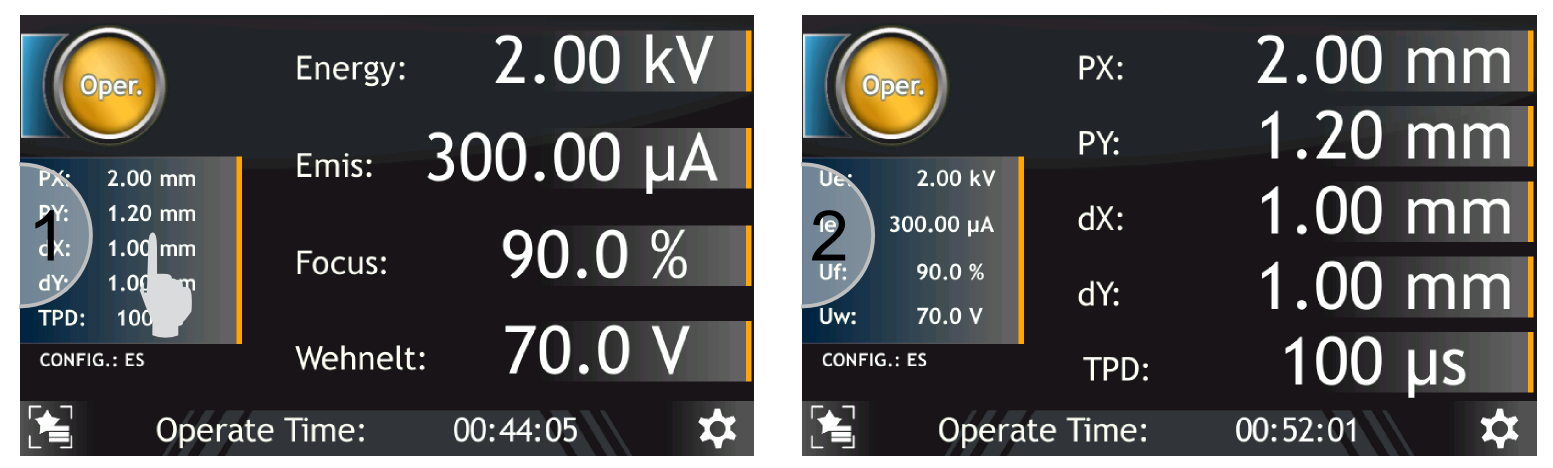
\includegraphics[width = 370 pt]{Figure/04/display.png}
\caption[Ukázka nastavení parametrů zdroje elektronů]{Ukázka nastavení parametrů zdroje elektronů a přepnutí do druhého menu. Převzato z~\cite{Manual}}
\label{04display}
\end{figure}

%princip změny polohy?
%
%\begin{figure}[htbp!]
%\centering
%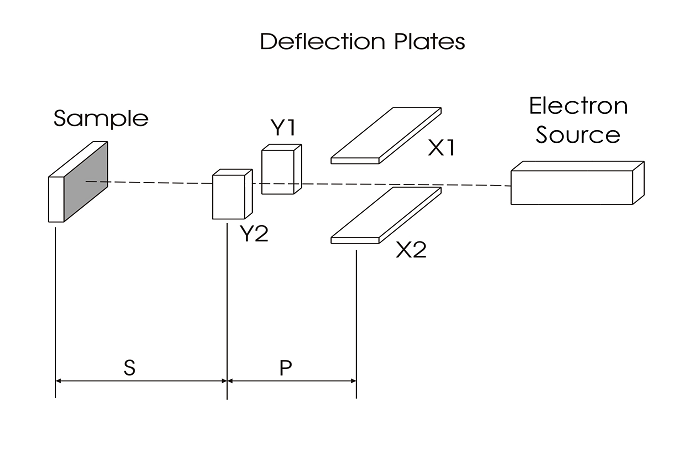
\includegraphics[width = 170 pt]{Figure/04/schema2.png}
%\caption{. Převzato z~\cite{Manual}}
%\label{04schema2}
%\end{figure}

Spuštění zdroje elektronů ES40-PS krok za krokem:
\begin{enumerate}
\item Po zapnutí napájení by měl být zdroj ponechán v režimu \textit{STAND-BY} alespoň 10 minut pro řádné zahřátí a stabilizaci katody
\item Pokud zdroj nebyl použit delší dobu následuje \textit{DEGAS} procedura
\item Následuje zapnutí do \textit{OPERATE} módu, ale pouze v případě je-li tlak v komoře nižší než $5 \times 10^{-6}$ mbar
\item Doporučené začínající hodnoty jsou: Energie = 3 kV, Emise = 100 $\mu$A, Fokusace = 70 \%, Wehneltovo napětí = 85 V, PX = PY = dX = dY = 0 mm
\end{enumerate} 


\textbf{DEGAS} procedura:
\begin{enumerate}
\item Před zapnutím do \textit{OPERATE} módu je nutné nastavit všechny napětí a proudy na minimum. 
\item Po zapnutí do \textit{OPERATE} módu je nutné nastavit následující parametry v daném pořadí: Energie = $2{,}00$ kV, Fokusace = $88{,}0$ \% a Wehneltovo napětí~=~$71{,}0$~V
\item Zvýšení Emise na $300{,}00 \ \mu$A 
\item S tímto nastavením by mělo zařízení pracovat 10 minut
\item Následně by měla být emise snížena na minimum a poté i zbývající napětí
\end{enumerate}
Během \textit{DEGAS} procedury by měly být parametry zvyšovány postupně se současnou kontrolou tlaku v komoře. Pokud dojde k náhlému poklesu vakua v komoře, mělo by být zařízení ponecháno se stávajícími parametry dokud nedojde k obnovení vakua.

Více podrobností k ovládání zdroje elektronů ES40-PS je popsáno v operačním manuálu ~\cite{Manual}.

\newpage
\chapter{Fokusace - teorie} 
\label{kapFok}

Fokusace a urychlování svazku byly realizovány pomoci elektronové optiky, soustavy elektrostatických čoček - několika cylindrických elektrod na které se přivádí různé napětí.  

Princip funkce elektrostatických čoček se dá ukázat na příkladě tzv. einzelových čoček - neurychlující fokusující soustavy třech cylindrických elektrod, ve které boční elektrody jsou pouze uzemněné a na elektrodu uprostřed je přivedeno napětí (Obr. \ref{einzel}). 
\begin{figure}[H]
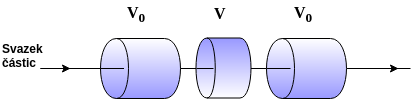
\includegraphics[width=.8\linewidth]{Figure/05/einzel.png}
\caption{Soustava třech elektrod s různým napětí.}
\label{einzel}
\end{figure}

Na Obr. \ref{pole} jsou schematický znázorněny siločáry elektrického pole vznikajícího v soustavě elektrod a chování svazku v tomto poli. Na prostřední elektrodu se v případě svazku elektronů dodává záporné napětí a vytváří se rozdíl potenciálů s každou s uzemněných okrajových elektrod. Po průchodu polem v rozmezí první a druhé elektrody svazek je zpomalen a rozptýlen v radiálním směru, dále po průletu druhou elektrodou svazek začíná být urychlován a stlačen radiálně, což vede k fokusaci do jednoho bodu, po proletění kterého, svazek znova defokusuje. Jelikož svazek je nejdřív zpomalen a potom urychlen, výsledná kinetická energie svazku po průchodu soustavou zůstává nezměněná. 
\begin{figure}[H]
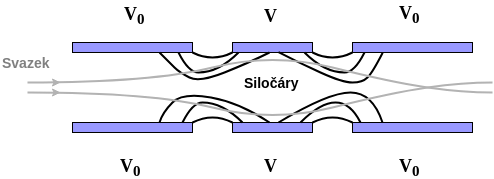
\includegraphics[width=.8\linewidth]{Figure/05/pole.png}
\caption{Schematické znázornění siločár elektrického pole v soustavě einzelových čoček.  }
\label{pole}
\end{figure}

Geometrie elektrod může být rozlišná a ovlivňuje fokusační vlastnosti soustavy, dalším důležitým parametrem působícím na chování svazku je napětí na elektrodách, v případě, že k dispozici je pouze soustava elektrod s určitou geometrii, polohu ohniska se dá zcela určit pomoci změny napětí na elektrodách. Při správném nastavení parametrů elektrostatické čočky nejenom fokusují svazek, ale také můžou ho urychlit, což jsme využili pro urychlování elektronového svazku v našem experimentu. 

Volbu geometrie a napětí na elektrodách jsme určili pomoci simulace soustavy v programu SIMION. 


\newpage
\chapter{Simulace fokusační soustavy}

úvod

\section{Koncept einzel lens}

Označení einzel lens se používá pro soustavu typicky tří cylindrických elektrostatických elektrod v řadě za sebou. Soustava slouží k fokusování iontového svazku ve vakuu pomocí specifického elektrického pole, které se běžně vytváří přivedením stejného napětí na krají dvě elektrody a odlišného napětí na prostřední elektrodu. Regulace napětí na prostřední elektrodě je pak dostačující ke kontrolování fokusačních vlastností aparatury, které ovšem celkově závisí i na geometrii elektrod a energii kontrolovaného svazku. Polarita použitého napětí se odvíjí od náboje fokusovaných iontů. V principu je totiž třeba vytvořit takový potenciálový rozdíl mezi elektrodami, aby mezi první a druhou elektrodou ionty překonávaly potenciálový kopec a mezi druhou a třetí elektrodou se vracely k nižšímu potenciálu. Potom vzhledem k zakřivení elektrického pole, které je dané geometrií elektrod, se trajektorie iontů nejprve odchýlý od směru svazku a zpomalý a následně jsou strženy zpět k ose svazku, aby se protly v jednom bodě, je-li poměr mezi napětími krajní a prostřední elektrody vhodně nastavený. To je možné díky tomu, že čím dále je konkrétní iont od osy svazku, tím více na něj působí zakřivení válcově symetrického pole. Energie svazku na výstupu by pak měla být nezměněna právě díky stejným hodnotám napětí na krajních elektrodách.\\

Na Obr. \ref{05schemaEinzelLens} lze vidět schématický nákres čočky, který ilustruje výše popsaný způsob fokusace. Ten jen demonstrovaný též Obr. \ref{05simulaceEinzelLens}, na kterém je výsledek simulace z programu SIMION, který znázorňuje potenciálové hladiny mezi elektrodami v rovině xy. Simulovaná konfigurace z obrázku má následující parametry: válcové elektrody mají průměr $d=35$~mm, krajní elektrody jsou dlouhé $l_o = 2$~mm, prostřední měří, $l_i = 26$~mm, tloušťka stěny válce je $t=1$~mm, napětí na elektrodách jsou $U_o = 5$~kV, $U_i = -18$ kV, energie svazku u zdroje je $E = 20$~keV. Svazek je nastaven tak, aby od zdroje divergoval. Tuto divergenci fokusační soustava zastavuje a směřuje trajektorie do vzdáleného ohniska. Na Obr. \ref{05simulaceEinzelLensPotencial} je pak výše potenciálové hladiny reprezentována třetí souřadnicí, což může pomoci k vytvoření intuitivní představy o průběhu fokusace.\\

\begin{figure}[htbp!]
\centering
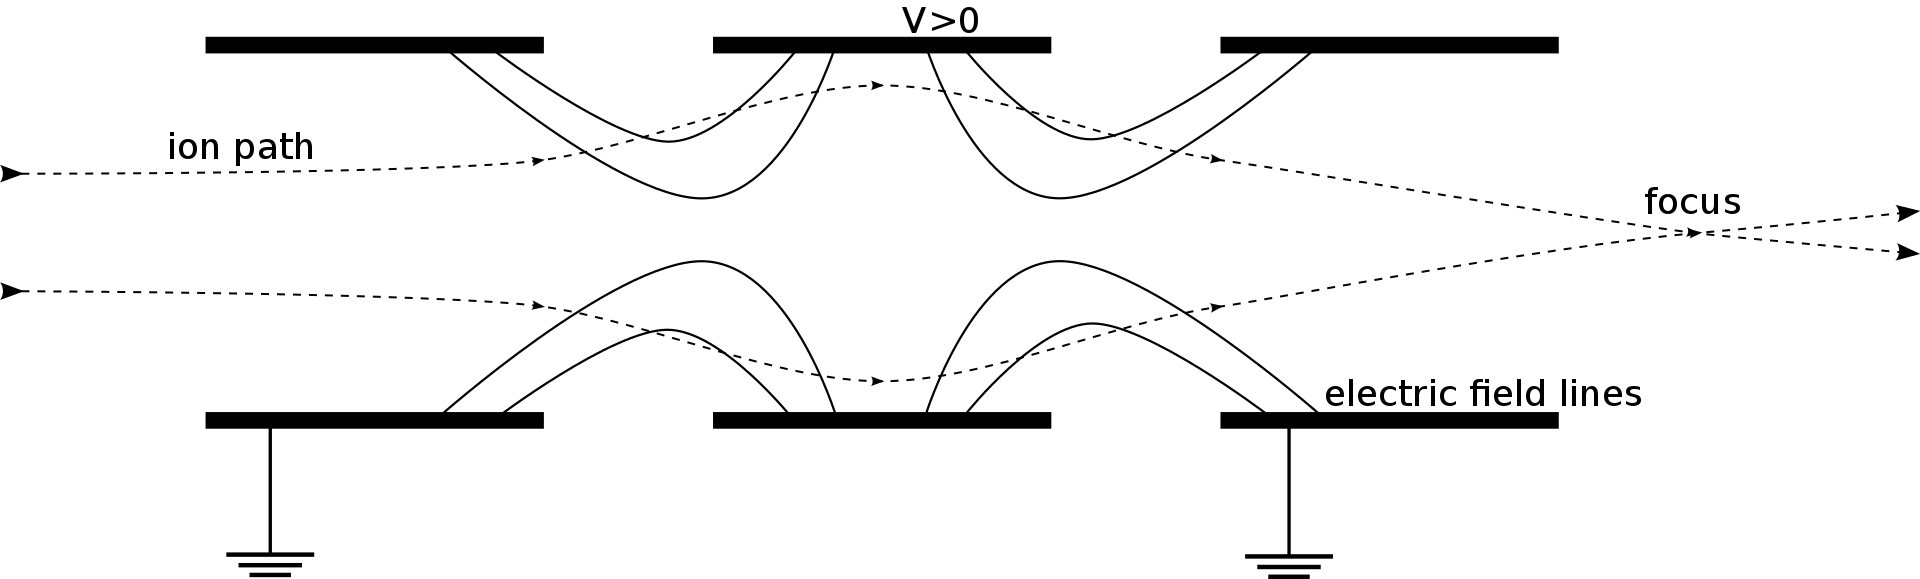
\includegraphics[width = 366 pt]{Figure/05/schema.png}
\caption{Caption.}
\label{05schemaEinzelLens}
\end{figure}

\begin{figure}[htbp!]
\centering
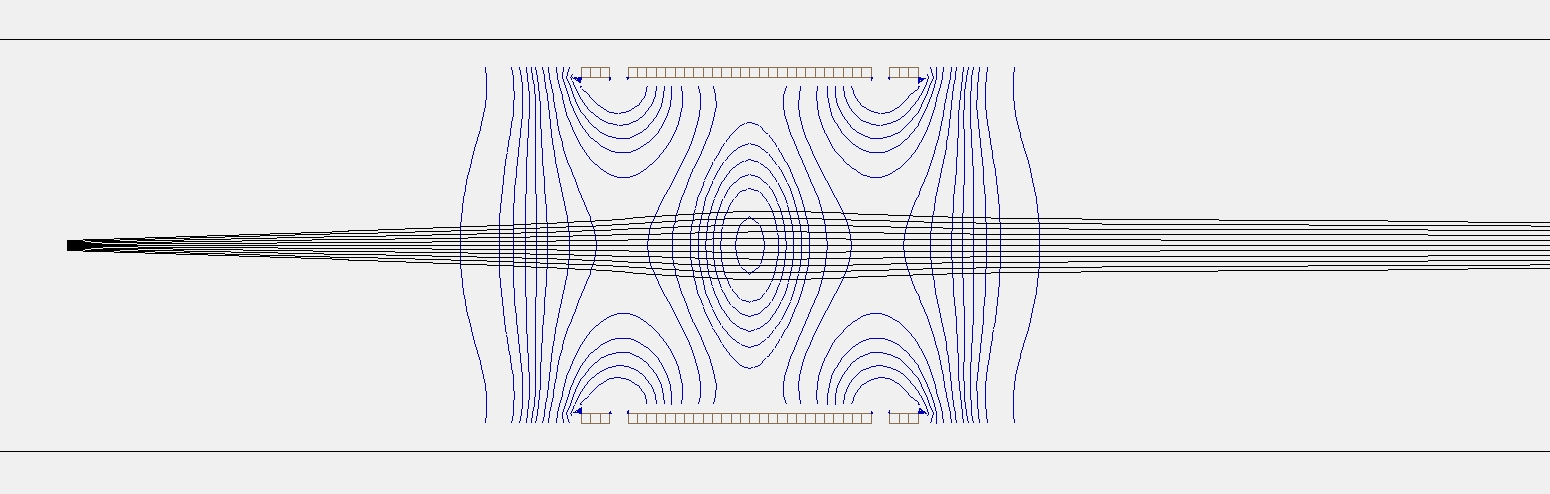
\includegraphics[width = 366 pt]{Figure/05/3a.jpg}
\caption{Caption.}
\label{05simulaceEinzelLens}
\end{figure}

\begin{figure}[htbp!]
\centering
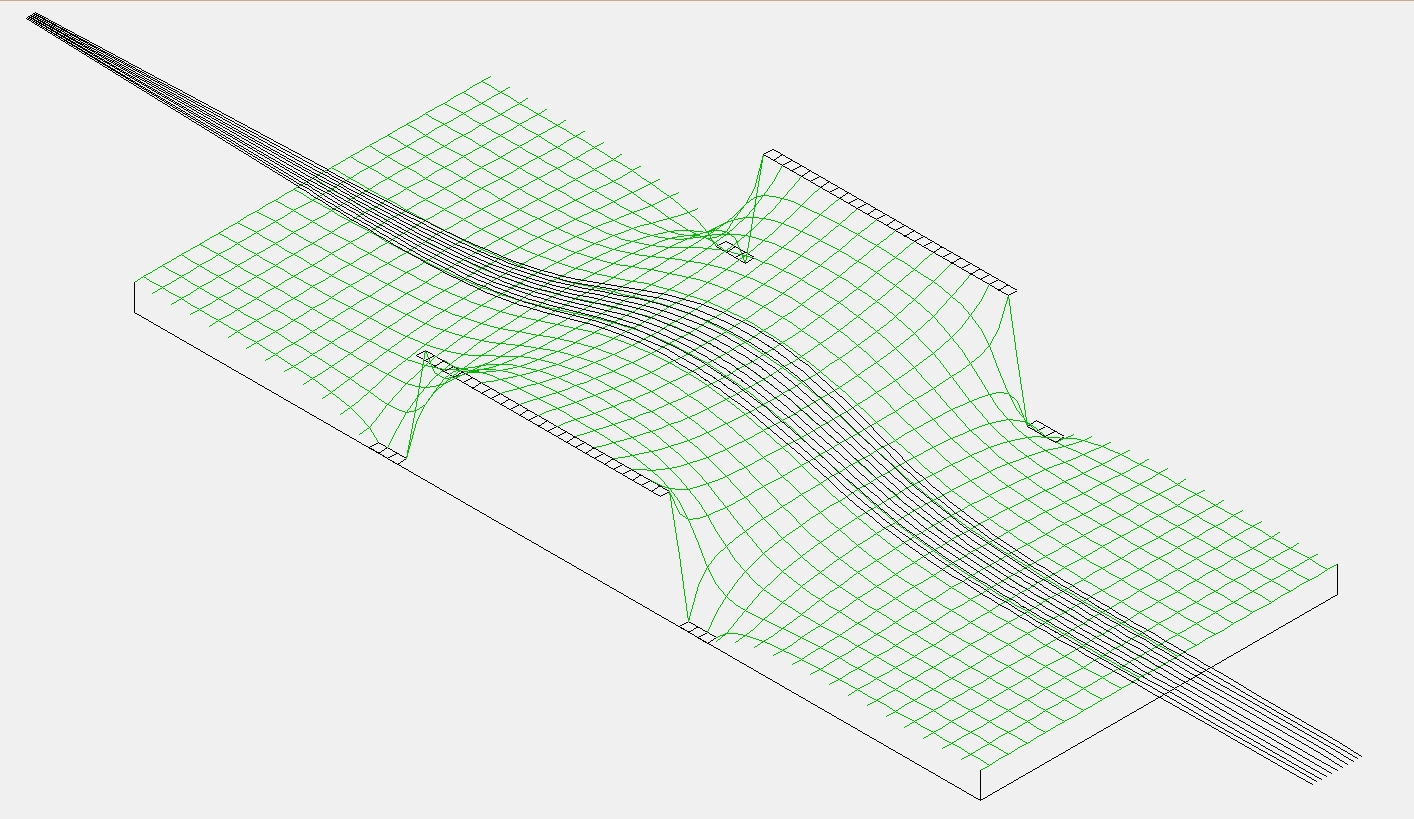
\includegraphics[width = 366 pt]{Figure/05/3b.jpg}
\caption{Caption.}
\label{05simulaceEinzelLensPotencial}
\end{figure}

Podobnou konfiguraci bylo původně v plánu použít k regulaci elektronového svazku z děla CRT obrazovky. Vzhledem k tomu, že se toto dělo nepodařilo zprovoznit, přešli jsme k novému konceptu, který zahrnoval konstrukci vlastního elektronového děla. Jako zdroj elektronů mělo sloužit wolframové vlákno a dělo mělo elektrony zároveň urychlovat a fokusovat pomocí soustavy čtyř elektrod, jejíž konfigurace se již odchylovala od typického uspořádání einzel lens, vycházela ovšem z podobných principů.\\

\section{Vlastní elektronové dělo}

Urychlování a fokusování elektronového děla měly zajišťovat čtyři válcové elektrody. Navrhovaná konfigurace byla podmíněna zejména dvěma požadavky:
\begin{itemize}
	\item k dispozici byly dva zdroje s napětím $~5$~kV (jeden lze rozdělit pro dvě elektrody) a jeden zdroj vysokého napětí $~80$~kV
	\item jako elektrody měly sloužit válečky nařezané z měděné trubky o průměru 3 cm různých délek
\end{itemize}

Nastavení napětí na elektrodách bylo motivováno myšlenkou, že elektrony, o nichž jsme předpokládali, že budou vylétávat z wolframového vlákna izotropně ve všech směrech s energiemi v řádech eV, je nejprve třeba urychlit v požadovaném směru a následně fokusovat a zároveň stanovit jejich finální energii, která měla původně dosahovat hodnot $~80$~keV. Proto napětí mezi první a druhou elektrodou vytvářela potenciálovou jámu, která měla elektrony strhávat správným směrem. Poslední tři elektrody pak měly společně tvořit soustavu podobnou einzel lens s tím rozdílem, že napětí na poslední elektrodě bude to nejvyšší a elektrony budou tak v poslední fázi fokusování zároveň urychleny na co nejvyšší energii. Na Obr. DOPLN je výsledek simulace navrhované konfigurace s těmito parametry:
\begin{itemize}
	\item Vzdálenost mezi elektrodami: $\Delta x = 2$ mm
	\item Geometrie elektrod: $d = 30$ mm, $l_0 = 40$ mm, $l_1 = 24$ mm, $l_2 = 26$ mm, $l_3 = 30$ mm
	\item Napětí na elektrodách: $U_1 = 1$ kV, $U_2 = 10$ kV, $U_3 = 1$ kV, $U_4 = 60$ kV
	\item Zdroj elektronů: bod umístěný 5 mm před první elektrodou, elektrony vylétávajícími do všech směrů s $E = 20$ eV
\end{itemize}

\begin{figure}[htbp!]
\centering
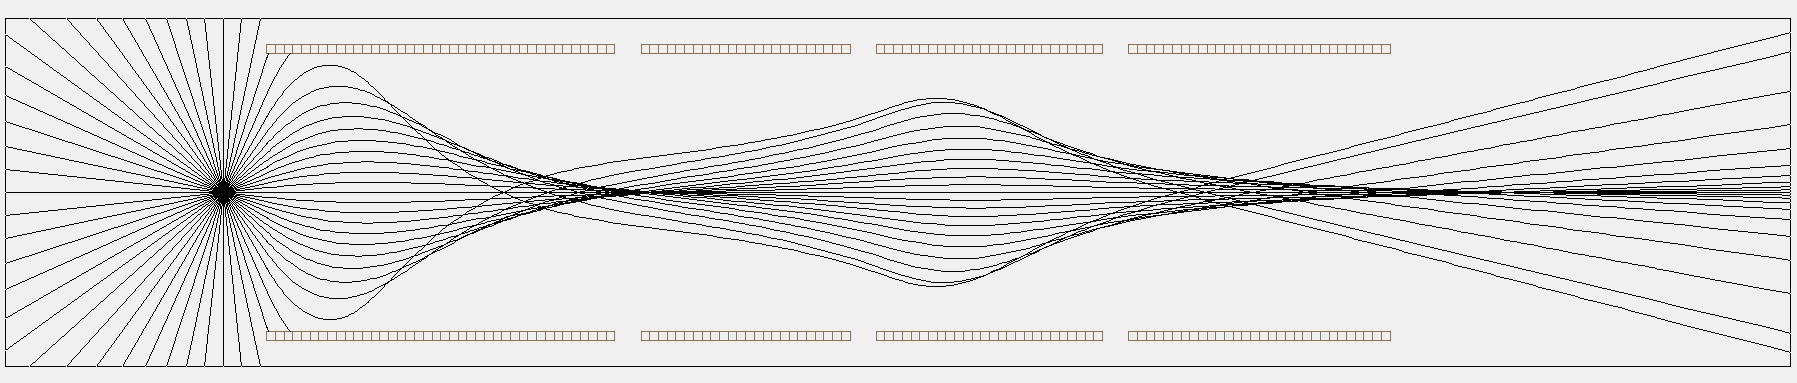
\includegraphics[width = 366 pt]{Figure/05/2a.jpg}
\caption{Caption.}
\label{05simulaceVlastniDelo}
\end{figure}

Konfiguraci lze ještě vylepšit jednoduše tím, že se wolframové vlákno umístí dovnitř první elektrody, jak ukazuje simulace na Obr. DOPLN., kde je zdroj elektronů umístěný 1 cm od levého kraje první elektrody. Nastavení simulace je jinak stejné jako u té předchozí, napětí na poslední elektrodě je ovšem $U_4 = 18$~kV, což se více blíží napětí, kterého jsme byli schopni dosáhnout bez probíjení. I tak se dalo očekávat, že alespoň na stínítku bychom mohli pozorovat stopu svazku. Nicméně ani s jednou konfigurací jsme ve vakuové komoře nakonec neuspěli. Další postup proto zahrnoval použítí zakoupeného průmyslového děla.\\

\begin{figure}[htbp!]
\centering
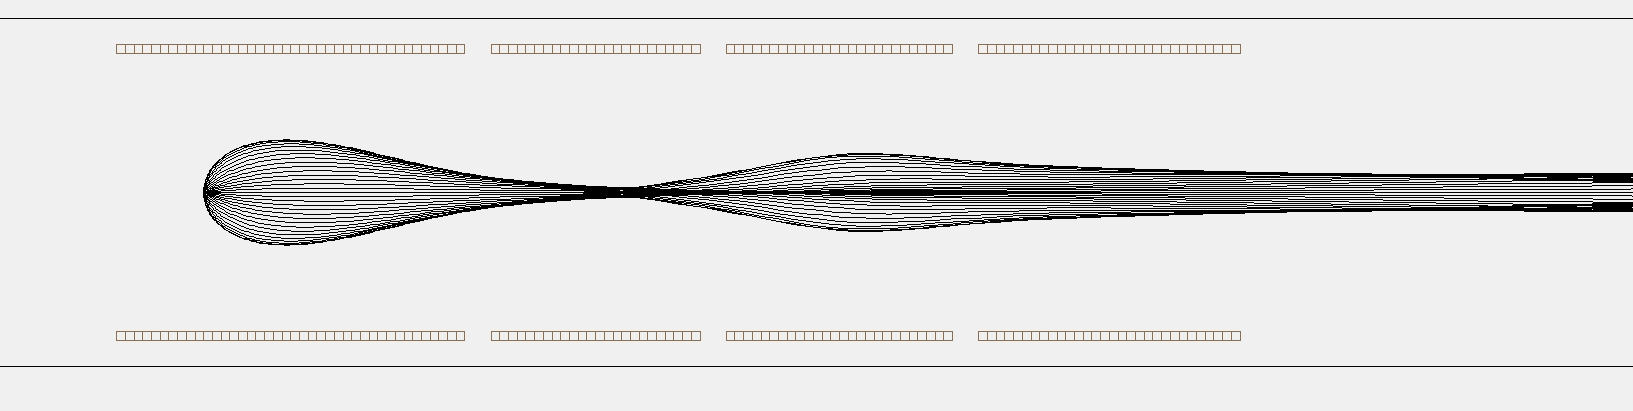
\includegraphics[width = 366 pt]{Figure/05/2c.jpg}
\caption{Caption.}
\label{05simulaceVlastniDeloWehnelt}
\end{figure}

\section{Urychlování svazku z průmyslového děla}

Zakoupené elektronové dělo bylo od výroby dostatečně dobře fokusované. Nejmenší možný průměr svazku uvedený výrobcem byl $d = 120$~$\mu$m ve vzdálenosti $l = 56$~mm. Proto fokusační soustava ztrácela svůj význam. Přesto však bylo třeba pro účely detekce svazek urychlit. Maximální energie svazku byla totiž $E = 5$~keV. Nakonec i možnost posouvat ohnisko svazku a tak jej fokusovat nebo defokusovat nezávisle na nastavení na průmylsovém děle se jevila jako zajímavá. Proto se finální fokusovací soustava skládala opět ze čtyř elektrod.\\

Elektrody byly tentokrát umístěny ve větší vzdálenosti od sebe, abychom omezili pravděpodobnost probíjení mezi nimy, ačkoliv jsme zcela s jistotou nevěděli, zdali k němu docházelo. Svazek z děla je v následujích simulacích reprezentován rovnoběžnými trajektoriemi dvou elektronů, které jej hypoteticky ohraničují. Průměr svazku je $d = 1$ mm a energie $E = 5$ keV. Ostatní parametry finální konfigurace jsou následující:
\begin{itemize}
	\item Vzdálenost mezi elektrodami: $\Delta x = 2$~mm
	\item Geometrie elektrod: $d = 30$~mm, $l_0 = 40$ mm, $l_1 = 24$ mm, $l_2 = 26$ mm, $l_3 = 30$ mm
	\item Napětí na elektrodách:
	\begin{enumerate}
		\item $U_1 = 1$ kV, $U_2 = 5$ kV, $U_3 = 1$ kV, $U_4 = 18$ kV
		\item $U_1 = 1$ kV, $U_2 = 15$ kV, $U_3 = 1$ kV, $U_4 = 18$ kV
		\item $U_1 = 1$ kV, $U_2 = 1$ kV, $U_3 = 1$ kV, $U_4 = 18$ kV
	\end{enumerate}
\end{itemize}

Ačkoliv to není z Obr. \ref{05simulaceFinalniKonfigurace} vzhledem k nepoměru mezi průměry svazku a elektrod zcela patrné, simulace ukazuje, že nastavováním napětí na druhé elektrodě lze teoreticky posouvat ohnisko, tudíž bychom mohli na stínítku pozorovat zvětšování, popř. zmenšování profilu svazku. Pro napětí $U_2 = 5$~kV se ohnisko nachází přibližně ve vzdálenosti $x = 178$ mm od levého kraje první elektrody. Pro napětí $U_2 = 15$~kV je to $x = 112$~mm a pro $U_2 = 1$~kV je $x = 204$~mm. Takový posun by se měl na stínítku v pevné vzdálenosti od zdroje projevit změnou průměru profilu řádově až v milimetrech, což by měl být pozorovatelný jev.\\

\begin{figure}[htbp!]
\centering
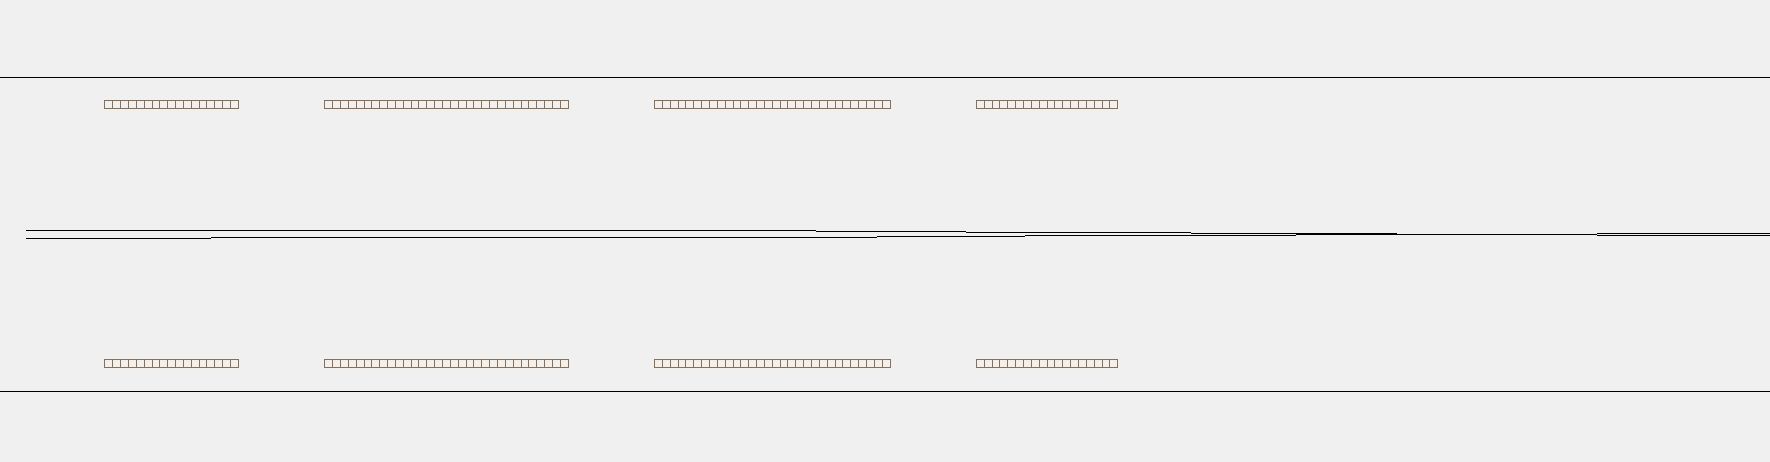
\includegraphics[width = 366 pt]{Figure/05/1a.jpg}
\vfill
\vfill
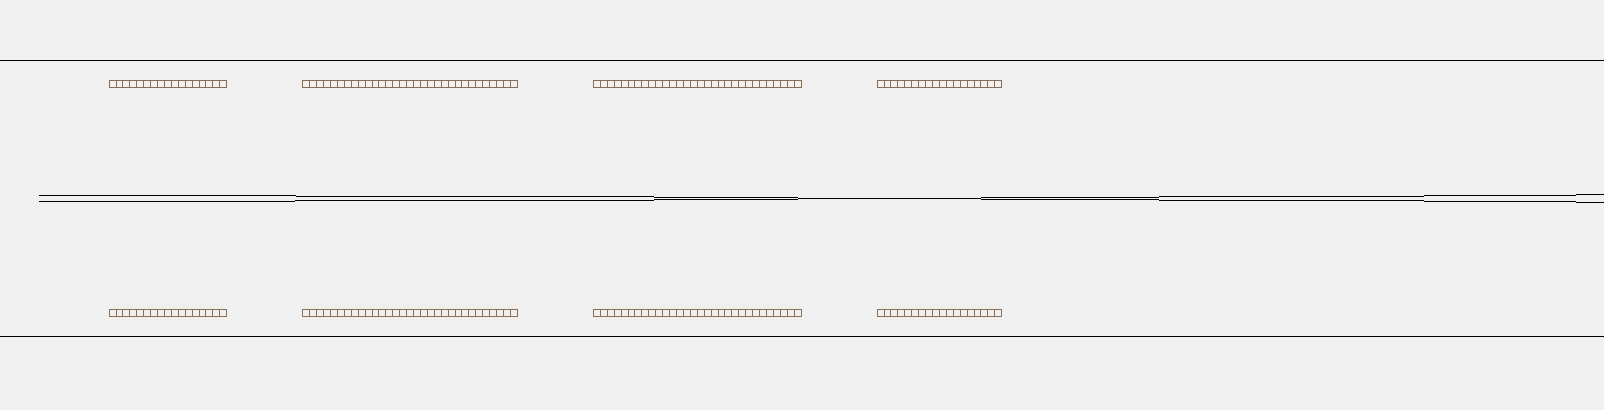
\includegraphics[width = 366 pt]{Figure/05/1b.jpg}
\vfill
\vfill
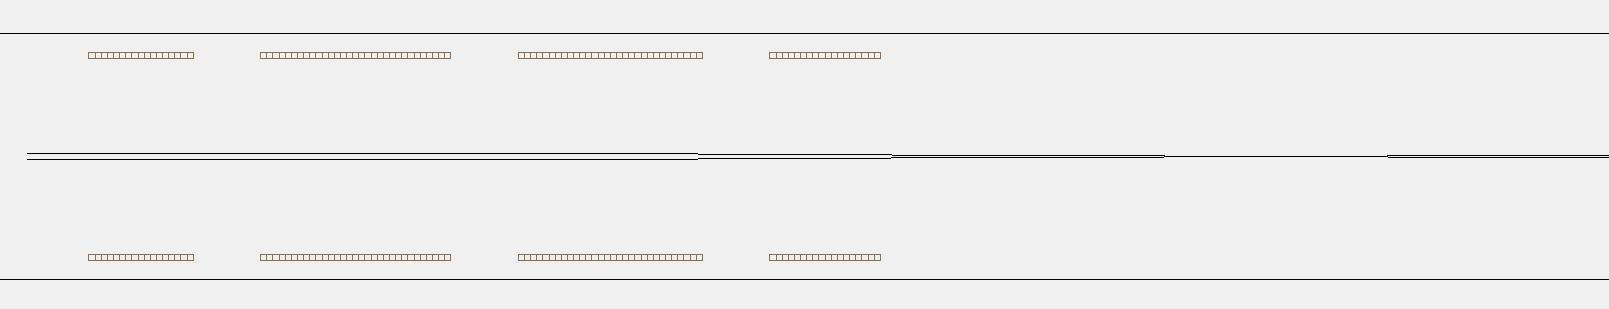
\includegraphics[width = 366 pt]{Figure/05/1c.jpg}
\caption{Caption.}
\label{05simulaceFinalniKonfigurace}
\end{figure}

\section{Zkouška děla se stínítkem}

\section{Závěr}

\end{document}

\newcommand{\fig}[4]{ 
	\begin{figure}[!ht]
		\centering
		\includegraphics[width=#1\linewidth]{Figure/07/#2.png}
		\caption[#3]{#4}
		\label{#2}
	\end{figure}
}

\interfootnotelinepenalty=10000
\renewcommand{\figurename}{Obr.}
\newcommand{\figref}[1]{\figurename \hspace{1 pt} \ref{#1}}

\newpage \clearpage

\chapter{Detekce svazku}
\label{kapMatej}

\section{Detekční technologie}
Po zvážení možností způsobu detekce elektronového svazku bylo jako optimální možnost zvoleno použití křemíkového pixelového detektoru X-CHIP03 vyvinutého v rámci FJFI ČVUT v Praze skupinou CAPADS. Ten by měl, jakožto detektor ionizujícího záření, dobře posloužit účelu, tedy zaznamenávání průletu elektronů. Další výhodou jeho použití byla možnost konzultace s týmem, který jej vytvořil. 

Vzhledem k monolitické technologii, v níž je detekční čip navržen, existuje spodní hranice pro energii detekovaných částic. Ta byla pro elektrony ze simulací stanovena na 80 keV - hodnotu, jíž bylo teoreticky elektronovým dělem dosáhnout. Vzhledem ke komplikacím, které se objevily během testování (dříve zmíněné vakuové výboje, ...) se nakonec bohužel podařilo dosáhnout energií maximálně 20 keV, které neprojdou vrstvou elektroniky do citlivé oblasti.

K vyřešení tohoto problému bylo navrženo využití konverzní vrstvy slitiny mědi a zlata. Tato tenká folie byla umístěna do cesty svazku před detektorem a při ozařování elektrony docházelo k emisi fotonů o podobné energii, které už nebyl problém detekovat. 

\section{Principy polovodičových detektorů}
\subsection{Pásová struktura}
Krystalické pevné látky se klasifikují jako vodiče, polovodiče a izolanty, přičemž kriteriem pro toto rozdělení je tzv. šířka zakázaného pásu. Ta vyplývá z pásové struktury (\figref{pasova_struktura}), tedy modelu, který popisuje energetické rozdělení elektronů v krystalu. 

\fig{1}{pasova_struktura}{Grafické znázornění pásové struktury.}{Grafické znázornění pásové struktury a) izolantu, b) polovodiče a c) vodiče. \cite{lutz1999semiconductor}}

Energetické spektrum samostatného elektronu je diskrétní, přičemž jednotlivé hladiny jsou určeny kvantovými čísly. Přidáváním dalších elektronů postupně dochází k rozštěpení hladin a při přechodu k makroskopickému popisu krystalu, je již třeba použít statistický model. Tím je pásová struktura, ve které se při velkém počtu elektronů původně diskrétní energetické hladiny shlukují do spojitých pásů - valenčního a vodivostního.

\textit{Valenční pás} obsahuje energie, při kterých jsou elektrony vázané v atomovém obalu a nemohou se volně pohybovat látkou. 

Přijme-li elektron dostatečnou energii, může přejít do \textit{vodivostního pásu}, ve kterém je v rámci krystalické mřížky delokalizovaný a může se podílet na vedení elektrického proudu.

Je-li krystalická látka vodivá, oba tyto pásy se překrývají a elektrony se tak mohou podílet na vedení proudu přirozeně. 

V případě izolantů jsou naopak pásy oddělené širokou oblastí energií, kterých elektrony nemohou nabývat - tzv. zakázaným pásem. Jeho šířka v prvním přiblížení\footnote{Roli zde hrají ještě další faktory, které oproti samotné ionizační energii šířku pásu zvětšují.} odpovídá ionizační energii atomů. 

Polovodiče mají sice ve své struktuře zakázaný pás také, jeho šířka je však na rozdíl od izolantů menší (řádově v jednotkách eV). To umožňuje korigovat jejich vlastnosti tak, aby podle potřeby vedly nebo nevedly elektrický proud. Když dojde k ionizaci atomu, vytvoří se v polovodiči dva efektivní nosiče náboje. Elektrony, které jsou na \figref{pasova_struktura} zobrazeny tečkami ve vodivostním pásu a díry, tedy absence elektronů v páse valenčním, zobrazené prázdnými kroužky.

Pohyb elektronů a děr společně vytváří celkový proud, přičemž elektrony se v materiálu pohybují rychleji\footnote{V křemíku je mobilita elektronů oproti děrám $\sim 3 \times$ větší.}.

\subsection{Vyprázdněná oblast}
Vlastnosti polovodičů mohou být zlepšeny tzv. dopováním. Při tomto procesu dochází k nahrazení malého množství atomů původní látky atomy s jiným (ale velmi blízkým) protonovým číslem. Tím vznikne přebytek nebo naopak nedostatek elektronů v krystalové mřížce\footnote{Polovodiče typu N mají přebytek elektronů, typu P přebytek děr.} a jsou tak apriori přítomny volné nosiče náboje.

Připojíme-li k sobe opačně dopované polovodiče, vznikne dioda a na jejím rozhraní tzv. vyprázdněná oblast, viz \figref{depleted}. Jde o místo, ze kterého jsou volné nosiče náboje vypuzeny vlivem přirozeně vzniklého elektrického pole. Pokud je navíc na diodu přivedeno napětí v závěrném směru, šířka vyprázdněné oblasti se zvětší.

\fig{.9}{depleted}{Přechod mezi P a N polovodiči.}{Přechod mezi P (nalevo) a N (napravo) polovodiči. Znaménka v kroužku značí volné nosiče náboje, které jsou v přítomnosti pole odpuzeny, nezakroužkovaná znaménka pak ionty ve vrcholech krystalické mřížky. Graf pod obrázkem zobrazuje průběh odpovídajícího potenciálu. \cite{spieler2005semiconductor_detector_systems}}

%Základním prvkem polovodičového detektoru je tzv. vyprázdněná oblast. Jde o místo s minimální koncentrací volných nosičů náboje, které vznikne v diodě při jejím zapojení v závěrném směru, viz \figref{depleted}. Na diodu je dále přivedeno tzv. biasovací napětí, které dále rozšiřuje vyprázdněnou oblast a navíc urychluje volné nosiče náboje, které by v ní vznikly.

\subsection{Vznik signálu}
%Pakliže vyprázdněnou oblastí proletí ionizující částice, předávají energii vázaným elektronům, které přejdou do vodivostního pásu. Při tomto přechodu vzniknou dva volné nosiče náboje: volný elektron a tzv. díra, tedy vakance ve valenčním páse, která se efektivně chová jako volný nosič náboje opačného znaménka. 

Pokud proletí elektricky nabitá částice vyprázdněnou oblastí předávají energii vázaným elektronům. Tak může dojít k předání energie dostatečné k přechodu vázaného elektronu do vodivostního pásu, tedy ionizaci atomu. Tím vznikne elektron-děrový pár.

Pokud má částice dostatečnou energii, mohou tyto páry vznikat podél celé její trajektorie, jak je vidět na \figref{particle-detection}. V elektrickém poli\footnote{Pole vzniká jako přirozený důsledek závěrného zapojení diody v kombinaci s biasovacím napětím.} driftují směrem ke sběrným elektrodám, které mohou bít umístěny na přední a zadní straně senzitivní oblasti.

Driftem elektronů a děr vzniká v materiálu proud, který je následně registrován jako signál. Jeho časový vývoj závisí například na typu nosiče\footnote{Elektrony se v křemíku pohybují $\sim 3 \times$ rychleji, než díry.} nebo na jeho aktuální poloze, pak záleží na tvaru elektrického pole v souladu se Shockley-Ramovým teorémem \cite{ramo1939}, \cite{shockley1938}. Příklad časové závislosti signálu je na \figref{pd_weightfield_mu}.

\fig{1}{particle-detection}{Znázornění elektron-děrových párů vzniklých ve vyprázdněné oblasti detektoru při průletu různých druhů ionizujících částic.}{Znázornění elektron-děrových párů vzniklých ve vyprázdněné oblasti detektoru při průletu různých druhů ionizujících částic.}

\fig{1}{pd_weightfield_mu}{Časový vývoj proudového signálu generovaného mionem o energii 1 GeV v pixelu křemíkového detektoru.}{Časový vývoj proudového signálu generovaného mionem o energii 1 GeV v pixelu křemíkového detektoru. Model z programu Weightfield2 \cite{2015weightfield}. Oranžová křivka značí proud indukovaný pohybem děr,modrá pohybem elektronů a černá celkový.}

\clearpage

\section{Pixelové detektory}
Polovodičové detektory se podle strukrtury uspořádání senzitivních oblastí dělí na stripové a pixelové. 

U prvních zmíněných je senzitivní oblast rozdělena na proužky (stripy), což je technologicky snazší varianta, detektor ale tak poskytuje informaci o zásahu pouze v jednom rozměru. 

Pixelové detektory naproti tomu mají senzitivní oblast tvořenou maticí pixelů, díky čemuž je jejich prostorové rozlišení apriori dvourozměrné. Pro účely skenování průřezu svazku je tedy pixelový detektor ideální volbou. Navíc se nabídla možnost využití pixelových detektorů vyvíjených na katedře, díky čemuž bylo možné v průběhu práce konzultovat jejich aplikaci s designéry.

V průběhu práce na experimentu se bohužel ukázalo, že výhody 2-D rozlišení není možné dostatečně využít, protože se nepodařilo svazek fokusovat do dostatečně malého průřezu a detektor tak vždy snímal pouze jeho část. Volbu pixelového detektoru však přesto považujeme vzhledem k detektoru za nejlepší možnou variantu.

%Jedním z typů polovodičových detektorů jsou pixelové, tedy matice nezávislých detekčních jednotek. Oproti druhé nejvýznamnější rodině - stripovým - nabízí apriori 2D rozlišení což je pro účel příčného skenování  elektronového svazku ideální. Tato potenciální výhoda bohužel nakonec zůstala nevyužita, protože se nepodařilo svazek dostatečně fokusovat a v místě detekce tak pokrýval větší plochu, než samotný detektor.\footnote{Je také možné, že k defokusaci svazku došlo využitím konverzní vrstvy.}

\section{X-CHIP03}
Pro skenování elektronového svazku byl v rámci tohoto projektu zvolen X-CHIP03 (\figref{xchip03_mp}). Jde o monolitický\footnote{V případě monolitických detektorů je na rozdíl od hybridních vyčítací část elektroniky umístěna ve stejném jednolitém objemu křemíku jako senzitivní vyprázdněná oblast.} pixelový detektor tvořený maticí 64x64 pixelů o rozměrech $4.2\times 5 \mathrm{mm}^2$. 

\fig{1}{xchip03_mp}{Model designu a fotografie detekčního čipu X-CHIP03.}{Model designu (vlevo) a fotografie (vpravo) detekčního čipu X-CHIP03, \cite{xchip03}.}

Detekční set-up, viz \figref{setup} se skládá z čipu umístěného na FURRy, PCB zprostředkující transfer fyzického signálu do USB portu, který je možné přímo připojit k počítači. Ke zpracování dat pak slouží software ASPIRE, přičemž obě zmíněné složky byly vyvinuty v rámci CAPADS. Celý set-up je umístěn na stojanu, který byl pro tento účel navržen a vytvořen ve 3-D tiskárně. Přechod mezi vakuem a notebookem vyčítajícím data byl zajištěn přes přechodku vakuové komory, na kterou byl z obou stran zajištěn rozpojený USB kabel.

\fig{1}{setup}{Experimentální detekční set-up.}{Experimentální detekční set-up. V pravé části se nachází detekční čip X-CHIP03, překrytý zlatavou konverzní folií. Větší PCB je FURRy, oranžové komponenty slouží jako stojánek, dále upevněný ve vakuové komoře. Z levé části rovněž vystupuje port USB.}

\label{chapter2}

\clearpage \pagebreak \newpage

\newpage
\chapter*{Metodika měření a analýza výsledků} % normalni kapitola \chapter{kapitola}
\addcontentsline{toc}{chapter}{Experimentální set-up a analýza výsledků}

\textit{Anežka Kabátová}\\
V této kapitole bude popsáno, jak probíhalo měření pomocí experimentálního set-upu, který byl již částečně představen v předchozím textu. Bude vysvětleno, proč jsme přistoupili k jednotlivým řešením a s jakými problémy jsme se potýkali. Nakonec budou interpretovány výsledky měření thresholdu pro produkci charakteristického záření konverzní vrstvy, demonstrován pohyb svazku a proveden odhad energie měřených fotonů.\\

\section{Metodika měření}
Při výběru detekční technologie na úplném počátku našeho experimentu jsme se nejvíce obávali nedostatečné energie elektronového svazku, jelikož zvolený X-CHIP03 má na povrchu několik necitlivých vrstev, kterými nízkoenergetické částice neprojdou. Jelikož jsou ale pixelové křemíkové detektory velice perspektivní, rozhodli jsme se riskovat případné problémy za cenu vysokého přínosu naším dovednostem. Tato obava se bohužel vyplnila, protože ani přes opakovanou snahu dosáhnout vyšších energií se nepodařilo zabránit náhodným výbojům v komoře, které by mohly detektor zničit.\\
Abychom získali detekovatelné částice, rozhodli jsme se použít konverzní vrstvu ze slitiny mědi a zlata, která pomocí excitace a následné deexcitace atomů uvnitř ní vyzařuje charakteristické záření. Toto záření má samozřejmě maximálně stejnou energii, jako elektronový svazek, ale díky rozdílnému mechanismu interakce fotonů a elektronů s látkou nemají problém projít až do citlivé oblasti čipu. Použitím konverzní vrstvy jsme ale přišli o informaci o původní energii částic, jelikož po dosažení thresholdu se objeví charakteristické záření, jehož energie podléhá pouze statistickým fluktuacím. Na druhou stranu jsme získali přibližnou informaci o energii detekovaných částic, kterou jsme mohli dále využít pro kontrolu orientační kalibrace detekčního čipu.\\
Detekční čip je, jak už bylo zmíněno, složen z matice 4096 pixelů. Každý funguje jako samostatná detekční jednotka, skládající se z vyprázdněné oblasti, v níž dochází ke vzniku volných nosičů náboje, a vyčítacího obvodu, v němž se na základě Shockley-Ramo teorému generuje z pohybujícího se náboje proud. Výstupem celého obvodu jsou jednotky analogově digitálního převodníku (ADC jednotky). Ty mají s energií původní částice spojitost, jelikož množství volných nosičů náboje, tedy i proud, jsou na ní závislé. K přiřazení energetické škály konkrétnímu pixelu se však musí provézt časově náročná kalibrace.\\
Pro účely tohoto experimentu kalibrace provedena nebyla, ale byly využity kalibrační křivky stejného detektoru. Ověření správnosti tohoto odhadu nám poskytuje právě energie charakteristických fotonů.\\
Konverzní vrstva, jak už bylo zmíněno, byla slitina zlata a mědi, bohužel v neznámém poměru. Charakteristické rentgenové záření pro různé elektronové hladiny obsahuje Tab. \ref{Tabulka1}.

\begin{table}
\begin{tabular}{|c|c|c|c|c|c|c|c|c|c|}
     \hline 
     Prvek & K$\alpha_1$ & K$\alpha_2$ & K$\beta_1$ & L$\alpha_1$ & L$\alpha_2$ & L$\beta_1$ & L$\beta_2$ & L$\gamma_1$ & M$\alpha_1$ \\ 
     \hline 
     Cu & 8.0 & 8.0 & 8.9 & 0.9 & 0.9 & 0.9 & - & - & - \\ 
     \hline 
     Au & 68.8 & 67.0 & 78.0 & 9.7 & 9.6 & 11.4 & 11.6 & 13.4 & 2.1 \\ 
     \hline 
     \end{tabular}
     \caption{Energie charakteristického záření pro jednotlivé elektronové hladiny v keV pro zlato a meď.}   
     \label{Tabulka1}
     \end{table}   

\section{Postup měření}
Provedená měření je možné rozdělit na dvě skupiny. Nejprve byla testována fokusace, což bylo rozebráno v příslušné kapitole. Konverzní vrstva částečně smývá informaci o poloze svazku, jelikož emitované fotony nemají stejný směr pohybu, jako původní elektrony. Pro účely testování fokusace tedy tento set-up není vhodný, a byl proto dočasně z komory odstraněn.\\
Nalezení ideální polohy pro měření zobrazuje video v příloze. Vidíme, že množství detekovaných detektorů se skokově zvýšilo.\\
Důležité pro ověření konceptu konverzní vrstvy bylo nalezení thresholdu pro výskyt charakteristického záření, čemuž jsme se věnovali v druhé části experimentu.

\section{Výsledky}
Z dostupných dat pozorujeme, že k nárůstu střední hodnoty pixelů došlo, nicméně ostrý threshold patrný není. To může být způsobeno rozdílnou energií elektronů ve svazku. Rostoucí odezva čipu v závislosti na napětí elektrody je na Obr. \ref{Obrazek_threshold}.

\begin{figure}[htbp!]
\centering
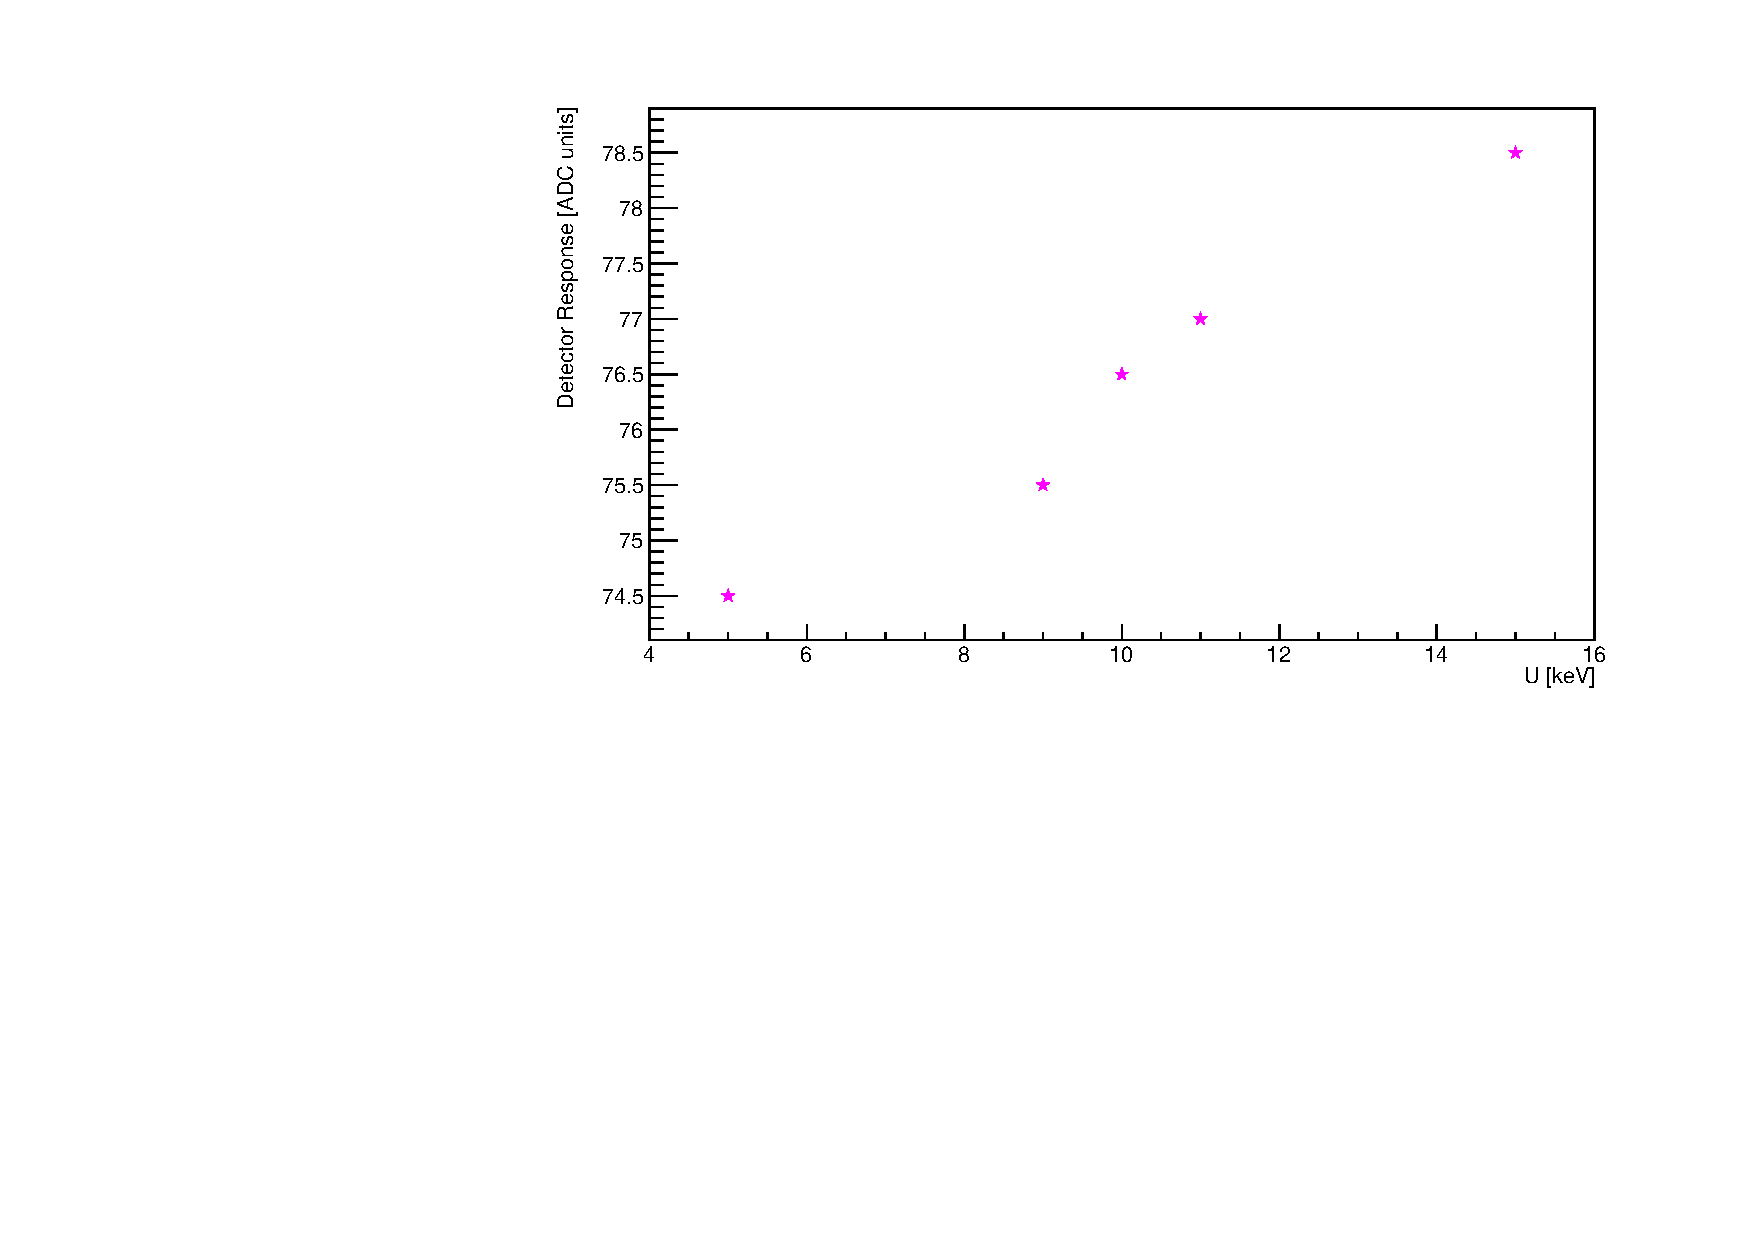
\includegraphics[scale = 0.7]{Figure/response.pdf}
 \caption{Střední odezva všech pixelů detektoru v jednotkách analogově-digitálního převodníku v závislosti na napětí elektrody elektronového děla.}
\label{Obrazek_threshold}
\end{figure}

Odezvu detektoru ve formě dvourozměrného histogramu lze najít na Obr. \ref{Obrazek_histo}. Souřadnicové osy odpovídají poloze jednotlivých pixelů v matici, jejich hodnota obsahuje informaci o střední odezvě daného pixelu.


\begin{figure}[htbp!]
\centering
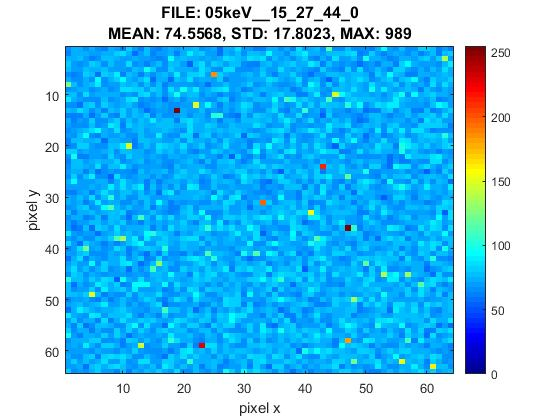
\includegraphics[width = 200 pt]{Figure/100_05keV__15_27_44_0.jpg}
\hfill
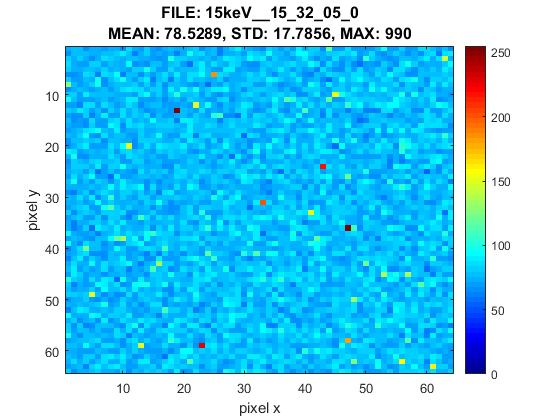
\includegraphics[width = 200 pt]{Figure/100_15keV__15_32_05_0.jpg}
 \caption{Dvourozměrné histogramy zobrazující momentální odezvu čipu pro nízké a vysoké napětí elektrody děla.}
\label{Obrazek_histo}
\end{figure}

Pomocí tohoto typu histogramu bylo také zjištěno, jaká byla přibližně energie detekovaných fotonů. Na detektoru stejného typu byla provedena energetická kalibrace jednotlivých pixelů, kterou lze využít k tomuto odhadu. Jak už bylo zmíněno, každý pixel v matici je svým způsobem originální kvůli nedokonalému výrobnímu procesu, jemuž se nedá předejít. Proto je třeba každému individuálnímu obvodu přiřadit lineární vztah mezi odezvou v ADC jednotkách a skutečnou energií. Dělá se tak pomocí známých spekter, jako jsou železo nebo plutonium. Nejprve jsou změřeny píky těchto spekter pomocí kalibrovaného detektoru, poté je jim přiřazena správná hodnota. Pokud je změřených píků dost, v tomto případě 4 (spektrum železa má jeden rozlišitelný pík, plutonium tři), lze těmito body proložit křivka a získat tak kýžený vztah.\\
Kalibrační křivku vybraného pixelu pro několik teplotních bodů zobrazuje Obr. \ref{Obrazek_kalibrace}.

 \begin{figure}[htbp!]
\centering
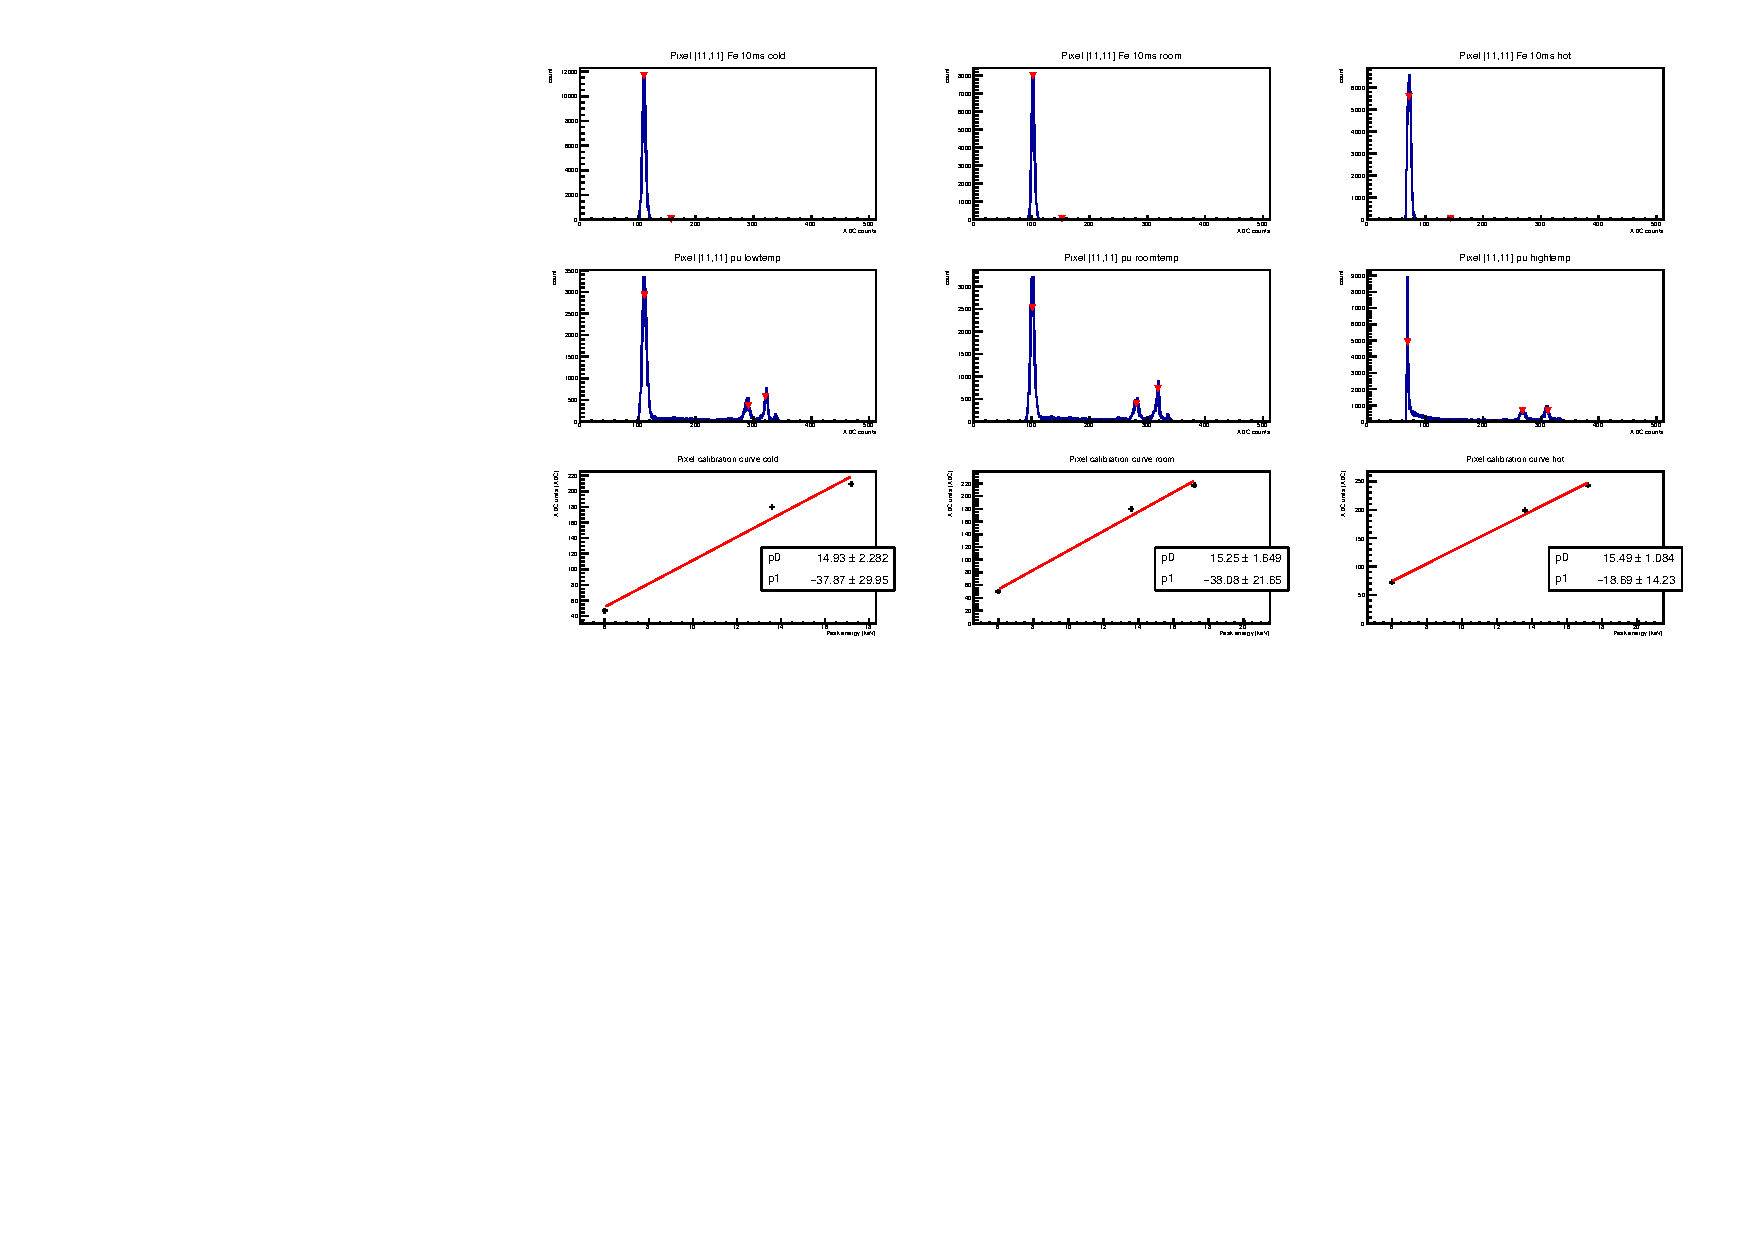
\includegraphics[scale = 0.85]{Figure/calibration.pdf}
 \caption{Kalibrace pixelu 11,11. Obrázky v prvních dvou řádcích zobrazují změřená spektra a v nich nalezené píky. V tomto případě byly pro kalibraci použity dva píky plutonia a jeden pík železa změřené při teplotě kolem 0$^{\circ}$, pokojové teplotě a teplotě kolem 60$^{\circ}$. Trojice obrázků ve spodním řádku pak zobrazuje kalibrační křivky a jejich parametry.}
\label{Obrazek_kalibrace}
\end{figure}

Pozorovaný rozdíl v ADC jednotkách mezi odezvou pixelu zasaženého elektronem a pozadím byl přibližně 80 ADC jednotek, což odpovídá podle kalibrační křivky zhruba 8 keV. To je v souladu s očekáváním, jelikož charakteristickému spektru mědi dominují fotony ze slupek K, které mají energii okolo 8 keV. 

 \begin{figure}[htbp!]
\centering
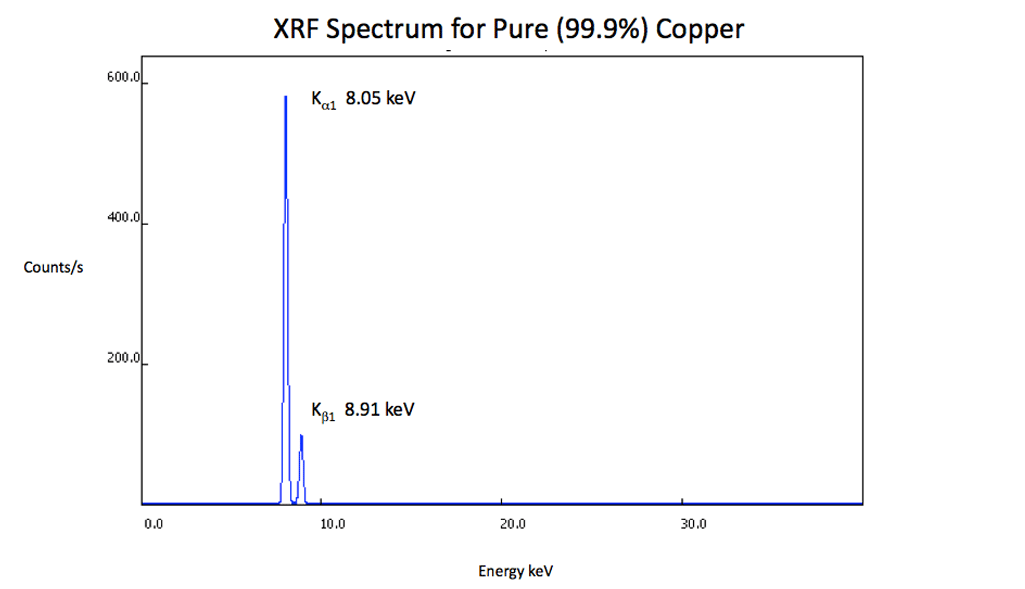
\includegraphics[scale = 0.4]{Figure/spektrum.png}
 \caption{Spektrum mědi s charakteristickými píky odpovídajícími fotonům emitovaných při deexcitaci na dvě vnitřní K-slupky.}
\end{figure}


\newpage
\chapter*{Závěr} % normalni kapitola \chapter{kapitola}
\addcontentsline{toc}{chapter}{Závěr}

Hlavním cílem této práce byla konstrukce zdroje elektronů, urychlovací a fokusovací aparatury spolu s detekčním zařízením a následné proměření vlastností celého zařízení a samotného elektronového svazku. 

V této práci byly nejprve představeny základy teorie elektronů a jejich chování ve vakuu. Dále byly popsány elektrické výboje a způsoby jejich eliminace. Ve třetí kapitole byly představeny metody získávání elektronů spolu s námi vytvořenými elektronovými zdroji a urychlovací aparaturou. V následující kapitole byl dále popsán zdroj elektronů ES40-PS a jeho technické parametry spolu s návodem na jeho ovládání. V páté kapitole byly popsány teoretické principy fokusace elektronového svazku. V následující kapitole jsme se seznámili se simulačním programem SIMION a jeho konkrétním využitím v našem experimentu spolu s výsledky měření fokusace elektronového svazku, které demonstrují funkčnost celé aparatury. V předposlední kapitole byly představeny principy detekce elektronů a námi použitý detektor spolu s jeho výrobou a technickými parametry. Nakonec byla představena metodika měření, naměřená data a výsledky analýzy dat, kde jsme konverzí elektronů na fotony pomocí slitiny mědi a zlata změřili spodní limit energie elektronů jako 8 keV.



\clearpage 
\addcontentsline{toc}{chapter}{Literatura} 


\bibliography{bibliografie}
\bibliographystyle{ieeetr}
%\bibliographystyle{plainnat}

\end{document}